\documentclass[12pt,a4paper]{report}  %紙張設定
\usepackage{xeCJK}%中文字體模組
%\setCJKmainfont{標楷體} %設定中文字體
\setCJKmainfont{MoeStandardKai.ttf}
%\newfontfamily\sectionef{Times New Roman}%設定英文字體
\newfontfamily\sectionef{Nimbus Roman}
\usepackage{enumerate}
\usepackage{amsmath,amssymb}%數學公式、符號
\usepackage{amsfonts} %數學簍空的英文字
\usepackage{graphicx, subfigure}%圖形
\usepackage{fontawesome5} %引用icon
\usepackage{type1cm} %調整字體絕對大小
\usepackage{textpos} %設定文字絕對位置
\usepackage[top=2.5truecm,bottom=2.5truecm,
left=3truecm,right=2.5truecm]{geometry}
\usepackage{titlesec} %目錄標題設定模組
\usepackage{titletoc} %目錄內容設定模組
\usepackage{textcomp} %表格設定模組
\usepackage{multirow} %合併行
%\usepackage{multicol} %合併欄
\usepackage{CJK} %中文模組
\usepackage{CJKnumb} %中文數字模組
\usepackage{wallpaper} %浮水印
\usepackage{listings} %引用程式碼
\usepackage{hyperref} %引用url連結
\usepackage{setspace}
\usepackage{lscape}%設定橫式
\lstset{language=Python, %設定語言
		basicstyle=\fontsize{10pt}{2pt}\selectfont, %設定程式內文字體大小
		frame=lines,	%設定程式框架為線
}
%\usepackage{subcaption}%副圖標
\graphicspath{{./../images/}} %圖片預設讀取路徑
\usepackage{indentfirst} %設定開頭縮排模組
\renewcommand{\figurename}{\Large 圖.} %更改圖片標題名稱
\renewcommand{\tablename}{\Large 表.}
\renewcommand{\lstlistingname}{\Large 程式.} %設定程式標示名稱
\hoffset=-5mm %調整左右邊界
\voffset=-8mm %調整上下邊界
\setlength{\parindent}{3em}%設定首行行距縮排
\usepackage{appendix} %附錄
\usepackage{diagbox}%引用表格
\usepackage{multirow}%表格置中
%\usepackage{number line}
%=------------------更改標題內容----------------------=%
\titleformat{\chapter}[hang]{\center\sectionef\fontsize{20pt}{1pt}\bfseries}{\LARGE 第\CJKnumber{\thechapter}章}{1em}{}[]
\titleformat{\section}[hang]{\sectionef\fontsize{18pt}{2.5pt}\bfseries}{{\thesection}}{0.5em}{}[]
\titleformat{\subsection}[hang]{\sectionef\fontsize{18pt}{2.5pt}\bfseries}{{\thesubsection}}{1em}{}[]
%=------------------更改目錄內容-----------------------=%
\titlecontents{chapter}[11mm]{}{\sectionef\fontsize{18pt}{2.5pt}\bfseries\makebox[3.5em][l]
{第\CJKnumber{\thecontentslabel}章}}{}{\titlerule*[0.7pc]{.}\contentspage}
\titlecontents{section}[18mm]{}{\sectionef\LARGE\makebox[1.5em][l]
{\thecontentslabel}}{}{\titlerule*[0.7pc]{.}\contentspage}
\titlecontents{subsection}[4em]{}{\sectionef\Large\makebox[2.5em][l]{{\thecontentslabel}}}{}{\titlerule*[0.7pc]{.}\contentspage}
%=----------------------章節間距----------------------=%
\titlespacing*{\chapter} {0pt}{0pt}{18pt}
\titlespacing*{\section} {0pt}{12pt}{6pt}
\titlespacing*{\subsection} {0pt}{6pt}{6pt}
%=----------------------標題-------------------------=%             
\begin{document} %文件
\sectionef %設定英文字體啟用
\vspace{12em}
\begin{titlepage}%開頭
\begin{center}   %標題  
\makebox[1.5\width][s] %[s] 代表 Stretch the interword space in text across the entire width
{\fontsize{24pt}{2.5pt}國立虎尾科技大學}\\[18pt]
\makebox[1.5\width][s]
{\fontsize{24pt}{2.5pt}機械設計工程系}\\[18pt]
\sectionef\fontsize{24pt}{1em}\selectfont\textbf
{
\vspace{0.5em}
cd2023 2b3-pj3bg6分組報告}\\[18pt]
%設定文字盒子 [方框寬度的1.5倍寬][對其方式為文字平均分分布於方框中]\\距離下方18pt
\vspace{1em} %下移
\fontsize{30pt}{1pt}\selectfont\textbf{BubbleRob八人對戰}\\
\vspace{1em}
\sectionef\fontsize{30pt}{1em}\selectfont\textbf
{
\vspace{0.5em}
BubbleRob Eight-Player Battle}
 \vspace{2em}
%=---------------------參與人員-----------------------=%             
\end{center}
\begin{flushleft}
\begin{LARGE}
\hspace{32mm}\makebox[5cm][s]
{指導教授:\quad 嚴\quad 家\quad 銘\quad 老\quad 師}\\[6pt]
\hspace{32mm}\makebox[5cm][s]
{班\qquad 級:\quad 四\quad 設\quad 二\quad 乙}\\[6pt]
\hspace{32mm}\makebox[5cm][s]
{學\qquad 生:\quad 莊\quad 雨\quad 薰\quad(41023203)}
\\[6pt]
\hspace{32mm}\makebox[5cm][s]
{\hspace{36.5mm}\quad 陳\quad 妤\quad 瑄\quad(41023204)}\\[6pt]
\hspace{32mm}\makebox[5cm][s]
{\hspace{36.5mm}\quad 陳\quad 靚\quad 芸\quad(41023205)}\\[6pt]
\hspace{32mm}\makebox[5cm][s]
{\hspace{36.5mm}\quad 陳\quad 澤\quad 瑜\quad(41023206)}\\[6pt]
\hspace{32mm}\makebox[5cm][s]
{\hspace{36.5mm}\quad 楊\quad 舒\quad 涵\quad(41023207)}\\[6pt]
\hspace{32mm}\makebox[5cm][s]
{\hspace{36.5mm}\quad 廖\quad 子\quad 儀\quad(41023208)}\\[6pt]
\hspace{32mm}\makebox[5cm][s]
{\hspace{36.5mm}\quad 鄭\quad 翊\quad 均\quad(41023210)}\\[6pt]
\hspace{32mm}\makebox[5cm][s]
{\hspace{36.5mm}\quad 徐\quad 佑\quad 寧\quad(41023255)}\\[6pt]
%設定文字盒子[寬度為5cm][對其方式為文字平均分分布於方框中]空白距離{36.5mm}\空白1em
\end{LARGE}
\end{flushleft}
\fontsize{18pt}{2pt}\selectfont\centerline{\makebox[\width][s]
{中華民國\hspace{3em} 
112 \quad 年\quad 6\quad 月}}
\end{titlepage}
\newpage
%=------------------------摘要-----------------------=%
\renewcommand{\baselinestretch}{1.5} %設定行距
\pagenumbering{roman} %設定頁數為羅馬數字
\clearpage  %設定頁數開始編譯
\sectionef
\addcontentsline{toc}{chapter}{摘~~~要} %將摘要加入目錄
\begin{center}
\LARGE\textbf{摘~~要}\\
\end{center}
\begin{flushleft}
\fontsize{14pt}{20pt}\sectionef\hspace{12pt}\quad 由於矩陣計算、自動求導技術、開源開發環境、多核GPU運算硬體等這四大發展趨勢,促使AI領域快速發展,藉由這樣的契機,將實體機電系統透過虛擬化訓練提高訓練效率,再將訓練完的模型應用到實體上。\\[12pt]

\fontsize{14pt}{20pt}\sectionef\hspace{12pt}\quad 此專題是運用實體冰球對打機,將其導入CoppeliaSim模擬環境並給予對應設置,將其機電系統簡化並運用Open AI Gym進行訓練,找到適合此系統的演算法後,再到CoppeliaSim模擬環境中進行測試演算法在實際運用上的可行性。並嘗試透過架設伺服器將CoppeliaSim影像串流到網頁供使用者觀看或操控。\\[12pt]

\end{flushleft}
\begin{center}
\fontsize{14pt}{20pt}\selectfont 關鍵字: 類神經網路、強化學習、\sectionef CoppeliaSim、OpenAI Gym
\end{center}
\newpage
%=--------------------Abstract----------------------=%
\renewcommand{\baselinestretch}{1.5} %設定行距
\addcontentsline{toc}{chapter}{Abstract} %將摘要加入目錄
\begin{center}
\LARGE\textbf\sectionef{Abstract}\\
\begin{flushleft}
\fontsize{14pt}{16pt}\sectionef\hspace{12pt}\quad Due to the four major development trends of multidimensional arrays  computing, automatic differentiation, open source development environment, and multi-core GPUs computing hardware. The rapid development of the AI field has been promoted. In view of this development, the physical mechatronic systems can gain machine learning efficiency through their simulated virtual system training process. And afterwards to apply the trained model into real mechatronic systems.\\[12pt]

\fontsize{14pt}{16pt}\sectionef\hspace{12pt}\quad This project is to use the physical air hockey to play machine, introduce it into the CoppeliaSim simulation environment and give the corresponding settings, simplify its electromechanical system and use Open AI Gym for training, find an algorithm suitable for this system, and then perform it in the CoppeliaSim simulation environment Feasibility of testing algorithm in practical application. And try to stream CoppeliaSim images to web pages for users to watch or manipulate by setting up a server.\\
\end{flushleft}
\begin{center}
\fontsize{14pt}{16pt}\selectfont\sectionef Keyword:  nerual network、reinforcement learning、 CoppeliaSim、OpenAI Gym
\end{center}

\newpage
%=------------------------目錄----------------------=%
\renewcommand{\contentsname}{\centerline{\fontsize{18pt}{\baselineskip}\selectfont\textbf{目\quad 錄}}}
\tableofcontents  %目錄產生
\newpage
%=------------------圖表目錄產生----------------------=%
\renewcommand{\listfigurename}{\centerline{\fontsize{18pt}{\baselineskip}\selectfont\textbf{圖\quad 目\quad 錄 }}}
\newcommand{\loflabel}{圖} %定義\loflabel 文字為圖
\renewcommand{\numberline}[1]{\loflabel~#1\hspace*{0.5em}}
\listoffigures
%\newcommand{\captioname}{圖}
%\newpage
%\renewcommand{\listtablename}{\centerline{\fontsize{18pt}{\baselineskip}\selectfont\textbf{表\quad 目\quad 錄 }}}
%\newcommand{\lotlabel}{表} %定義\lotlabel 文字為表
%\renewcommand{\numberline}[1]{\lotlabel~#1\hspace*{0.5em}}
%\listoftables

\end{center}
%=-------------------------內容----------------------=%
\chapter{目標}
接續專案二,對雙輪車進行設計改良,以提升行進與對戰效能,採用CAD進行場景與多輪車零組件設計後,轉入足球場景中以鍵盤arrow keys與wzas等按鍵進行控制,對陣雙方每組將有四名輪車球員,且每兩人在同一台電腦上操作。
球賽計分系統必須採.ttm格式建立(0~99),使能通用於各類場景計數之用,並可擴增至三位數計分。除了採用LED顯示計分外,另外以建立機械轉盤傳動計分系統。

\section{規格}
\begin{tabular}{p{8cm}}
  \textbf{足球規格:白色,直徑0.1m,重量0.5kg} \\
  \textbf{足球場地:長4m x 寬2.5m} \\
  \textbf{球門規格:長0.6m,高0.3m,寬0.1m} \\
  \textbf{球員尺寸範圍:長寬高各0.2m,重量5kg} \\
\end{tabular}

\section{規則}
\begin{tabular}{p{8cm}}
  \textbf{遊戲規則如下:} \\
  \textbf{雙方球員各別控制,進球門得一分} \\
  \textbf{在規定時間內得最多分者獲勝} \\
  \textbf{進球後,球會重新從中間開始} \\
\end{tabular}
\begin{figure}
  \begin{center}
    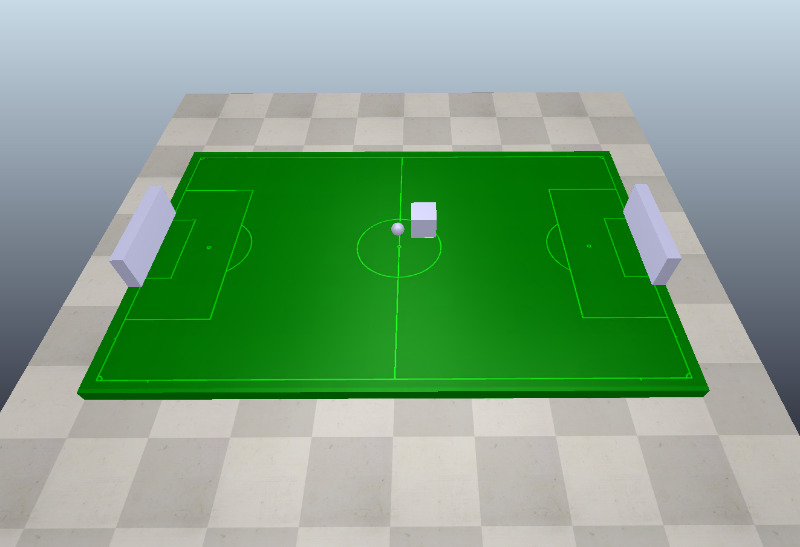
\includegraphics[width=0.5\textwidth]{football_field.png}
  \end{center}
  \caption{足球場景}
  \label{fig:photo}
\end{figure}

\chapter{球員}
\section{繪圖}
\newpage
\section{組裝}
\begin{figure}[h]
  \begin{center}
    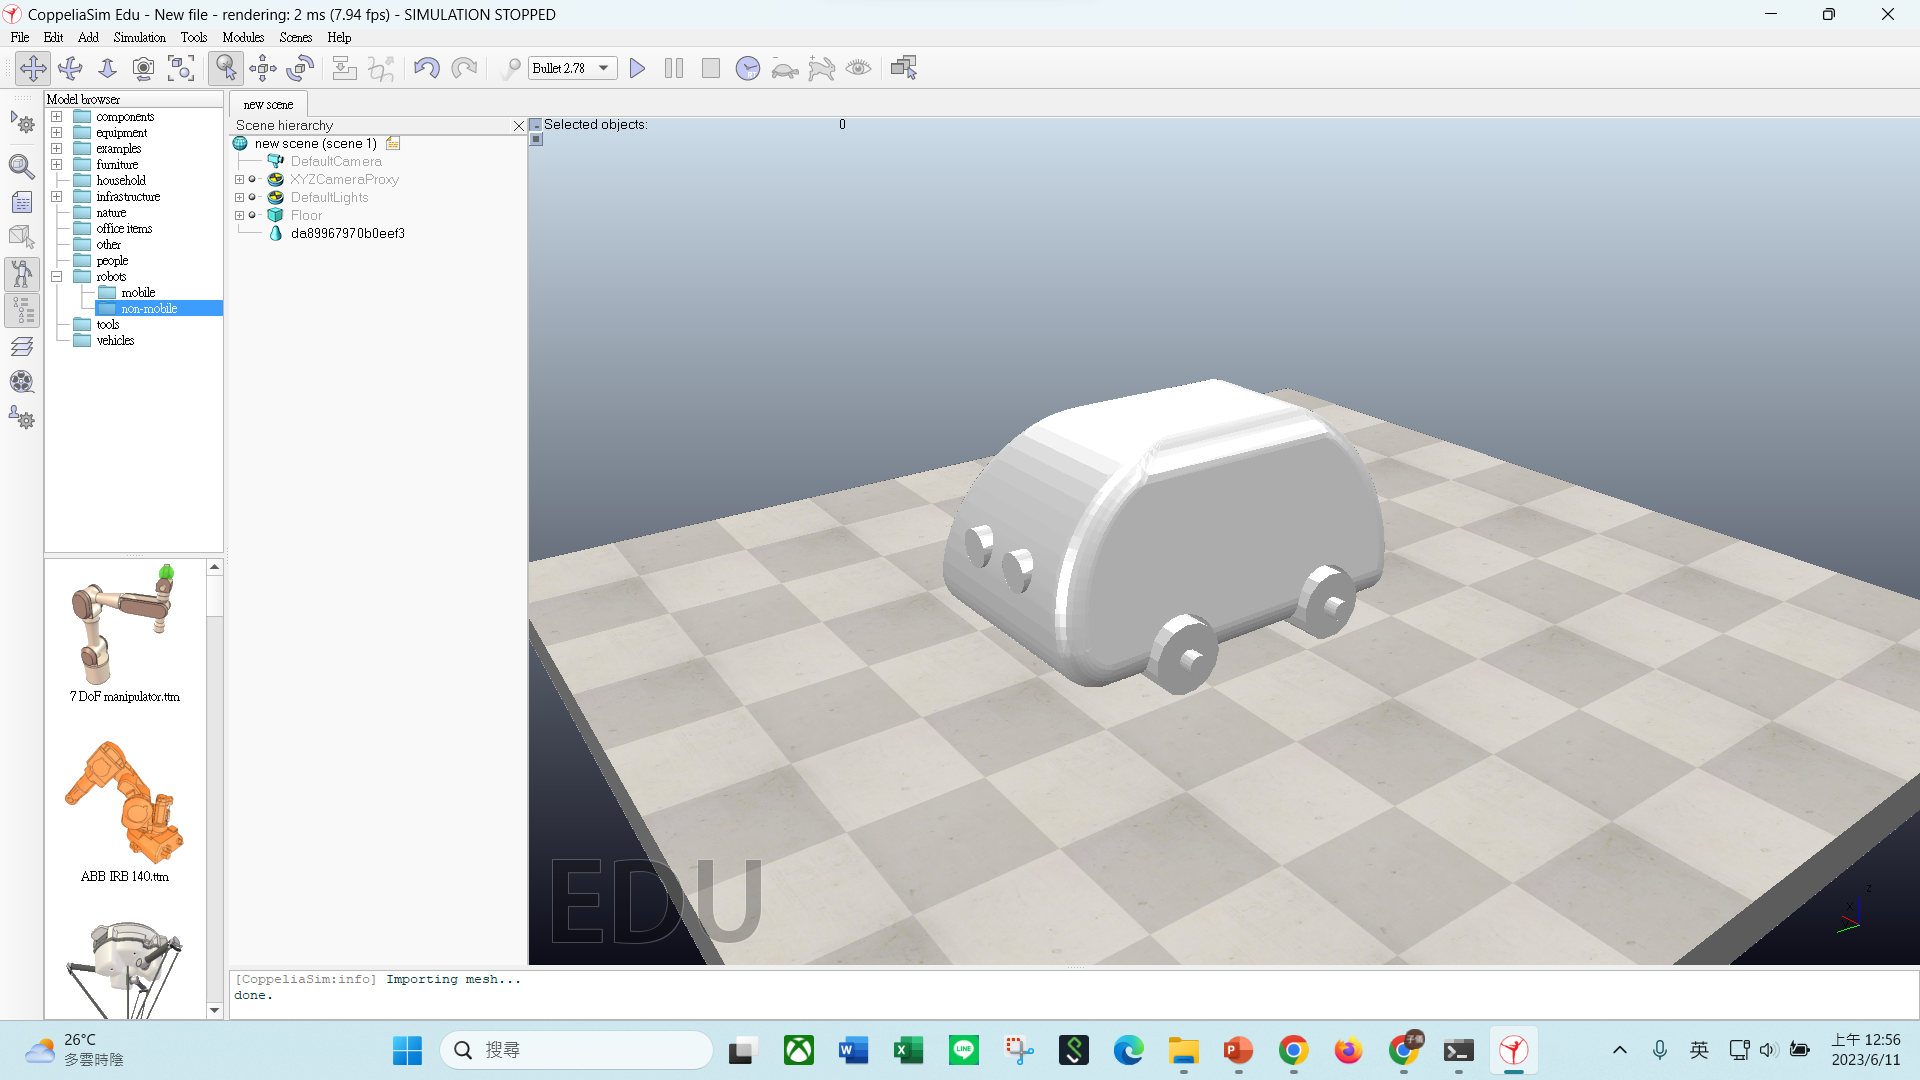
\includegraphics[width=0.5\textwidth]{球員組裝_1.png}
  \end{center}
  \caption{導入球員STL檔}
  \label{fig:photo}
\end{figure}
\begin{figure}[h]
  \begin{center}
    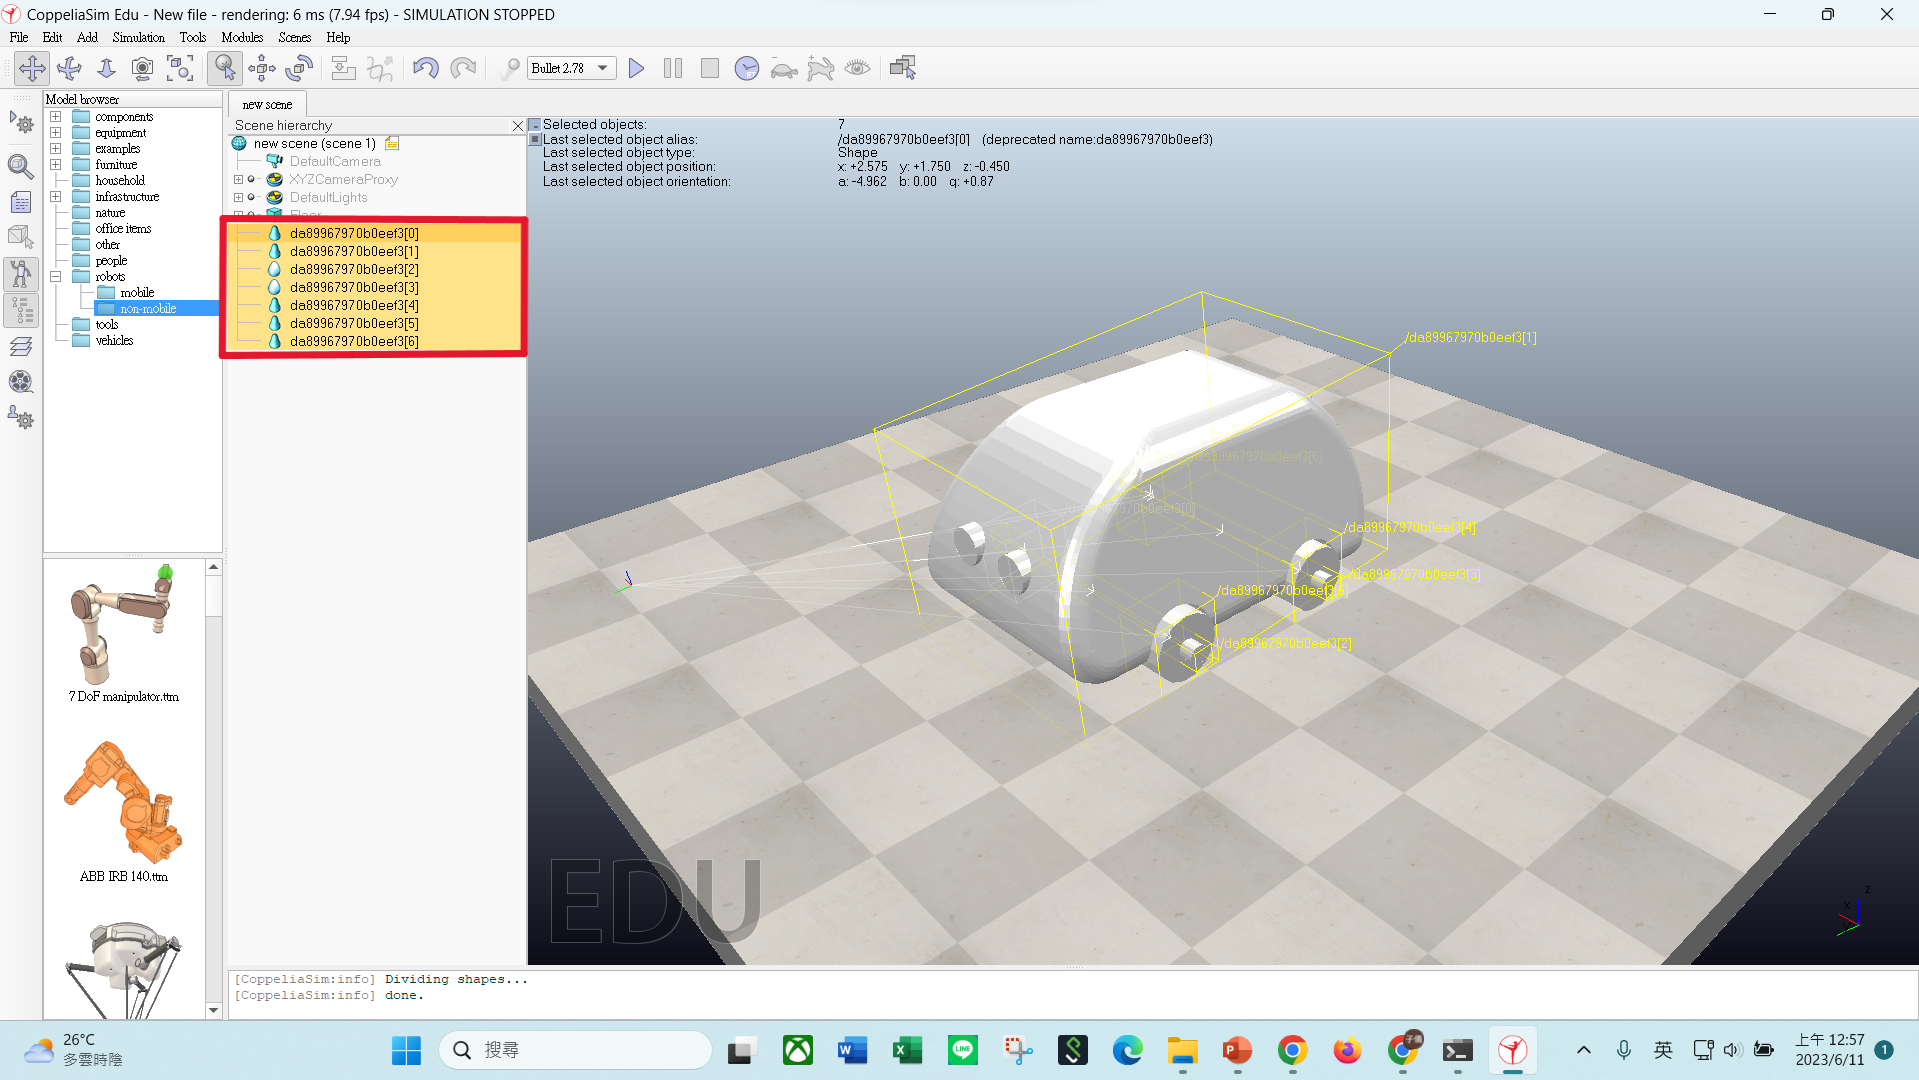
\includegraphics[width=0.5\textwidth]{球員組裝_2.png}
  \end{center}
  \caption{爆炸分解}
  \label{fig:photo}
\end{figure}
\begin{figure}[h]
  \begin{center}
    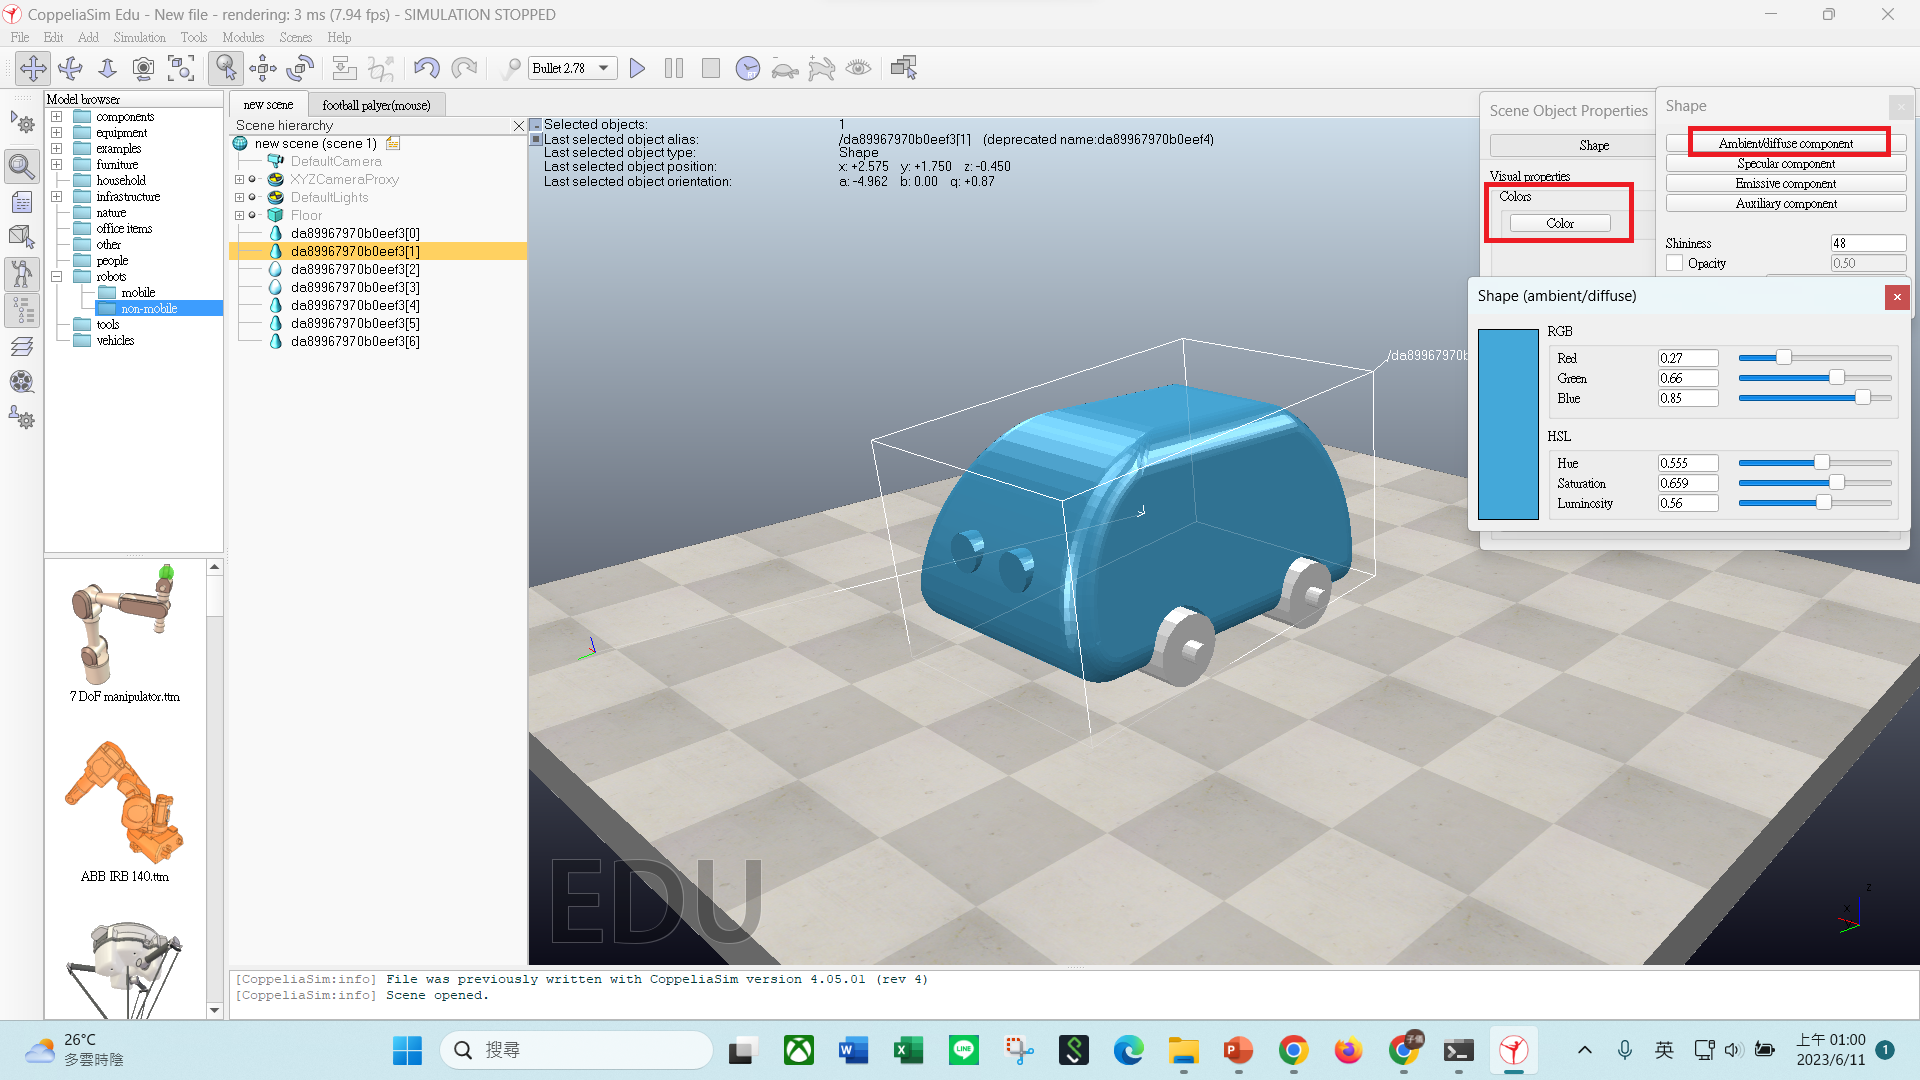
\includegraphics[width=0.5\textwidth]{球員組裝_3.png}
  \end{center}
  \caption{更改顏色}
  \label{fig:photo}
\end{figure}
\newpage
\begin{figure}[h]
  \begin{center}
    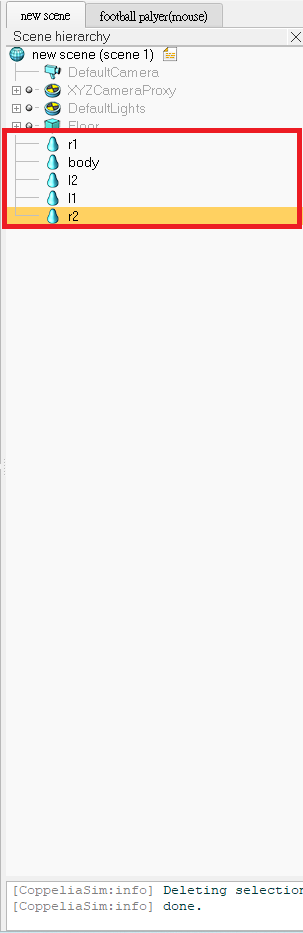
\includegraphics[width=0.5\textwidth]{球員組裝_4.png}
  \end{center}
  \caption{更改物件名稱}
  \label{fig:photo}
\end{figure}
\begin{figure}[h]
  \begin{center}
    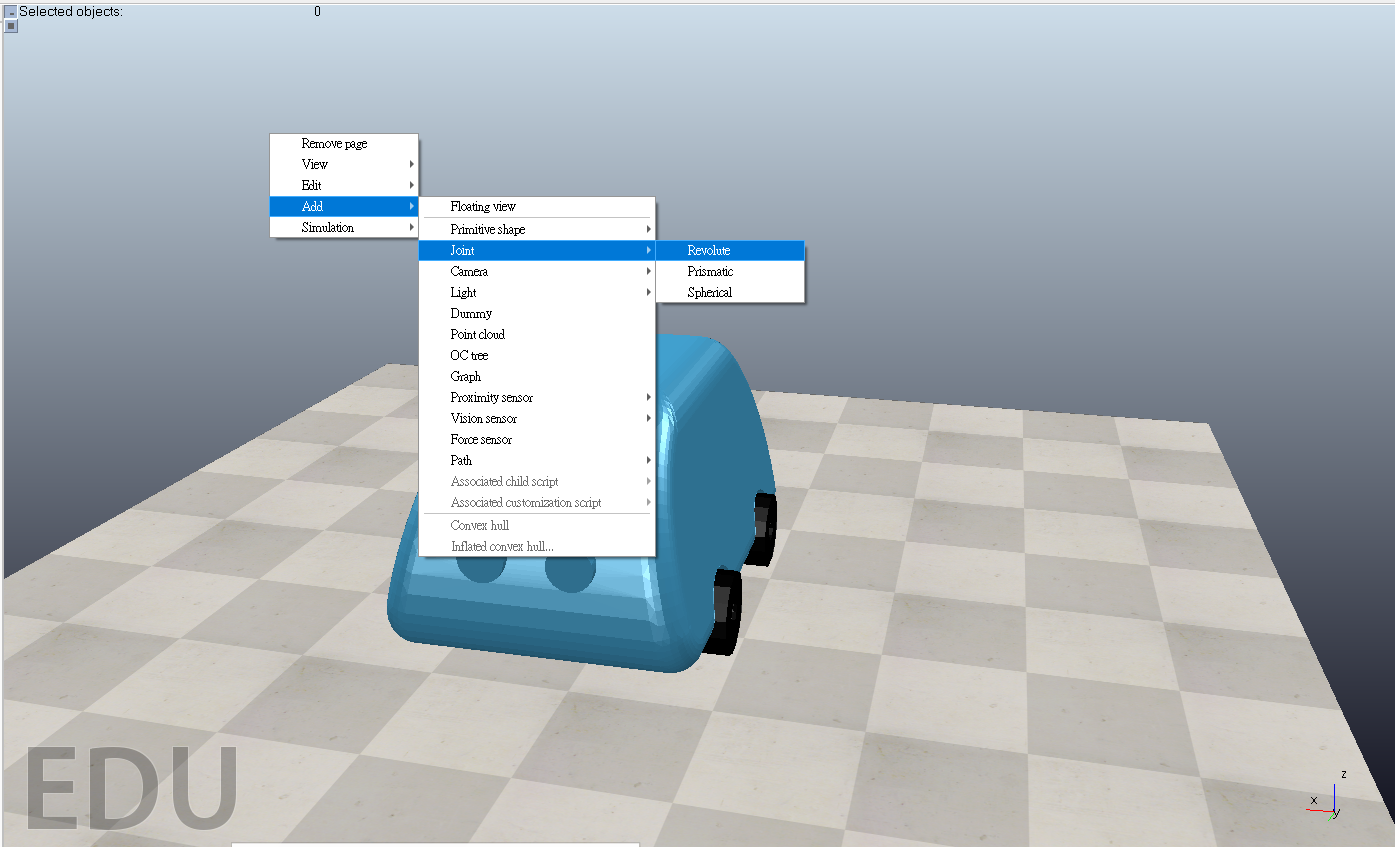
\includegraphics[width=0.5\textwidth]{球員組裝_5.png}
  \end{center}
  \caption{新增Joint}
  \label{fig:photo}
\end{figure}
\begin{figure}[h]
  \begin{center}
    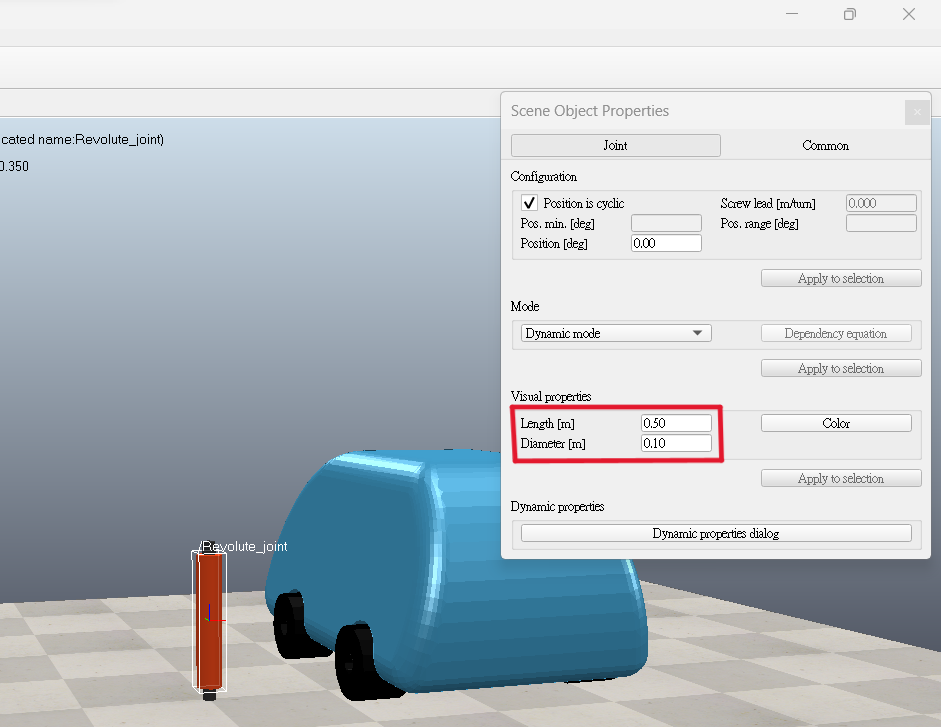
\includegraphics[width=0.5\textwidth]{球員組裝_6.png}
  \end{center}
  \caption{調整Joint大小}
  \label{fig:photo}
\end{figure}
\newpage
\begin{figure}[h]
  \begin{center}
    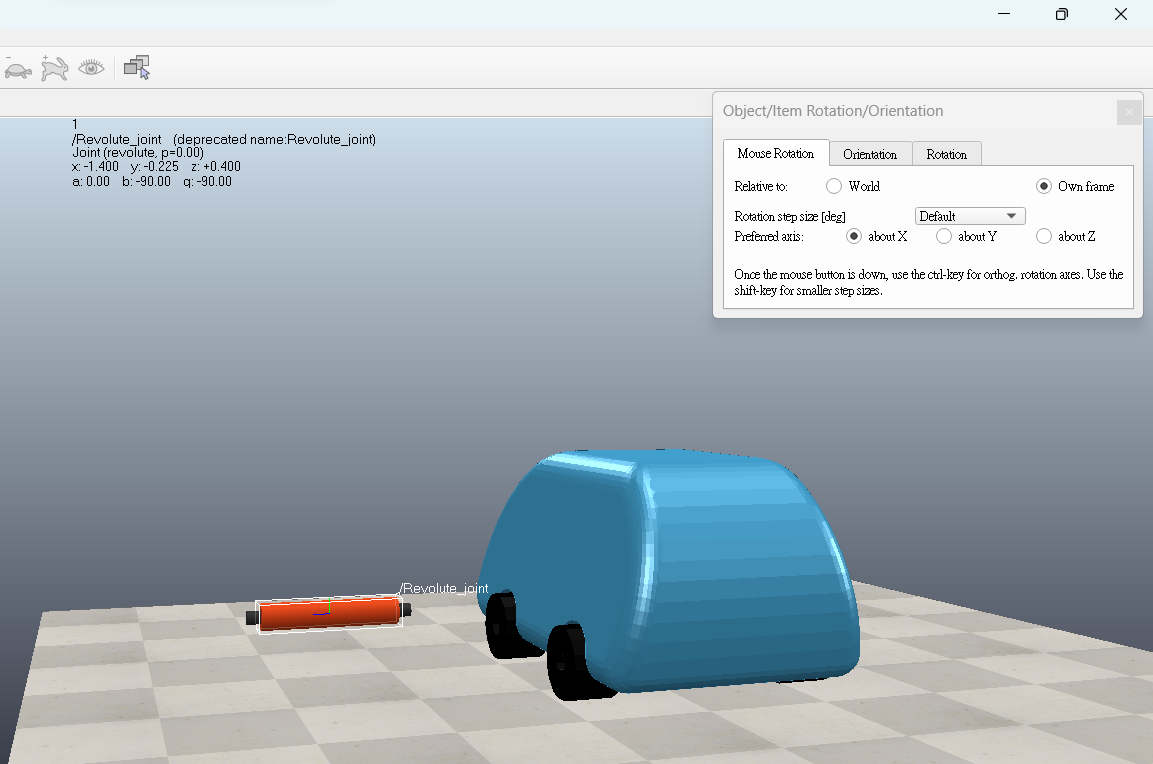
\includegraphics[width=0.5\textwidth]{球員組裝_7.png}
  \end{center}
  \caption{繞X軸旋轉,使Joint與物件平行}
  \label{fig:photo}
\end{figure}
\begin{figure}[h]
  \begin{center}
    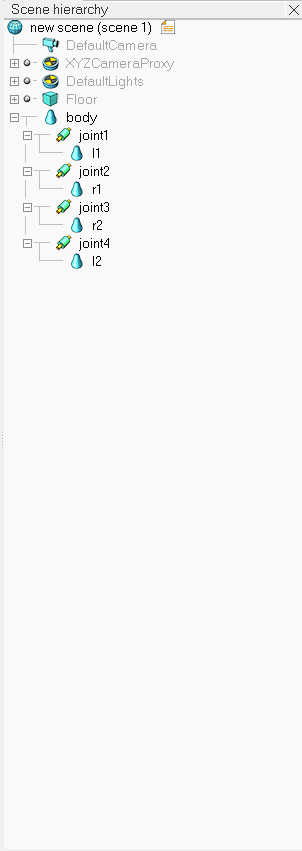
\includegraphics[width=0.5\textwidth]{球員組裝_8.png}
  \end{center}
  \caption{物件相互依附}
  \label{fig:photo}
\end{figure}
\begin{figure}[h]
  \begin{center}
    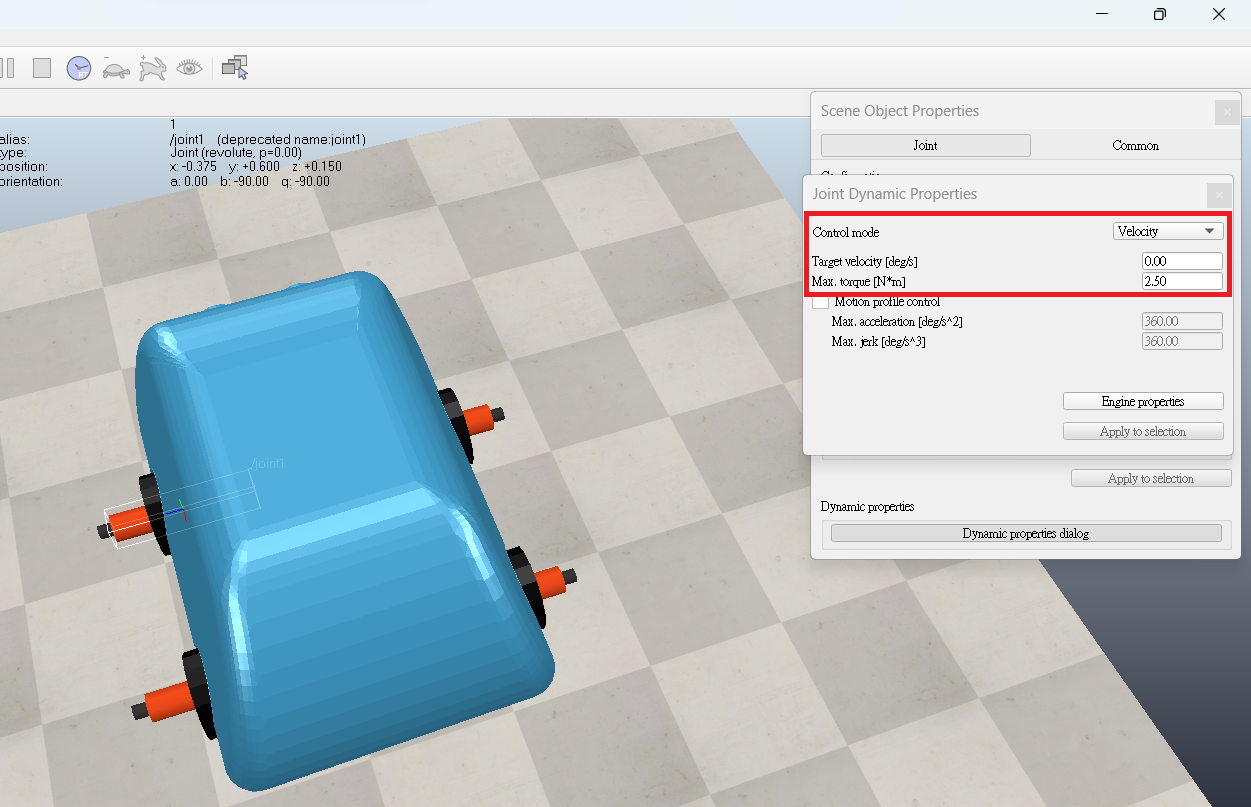
\includegraphics[width=0.5\textwidth]{球員組裝_9.png}
  \end{center}
  \caption{調整物件傳動參數}
  \label{fig:photo}
\end{figure}
\begin{figure}[h]
  \begin{center}
    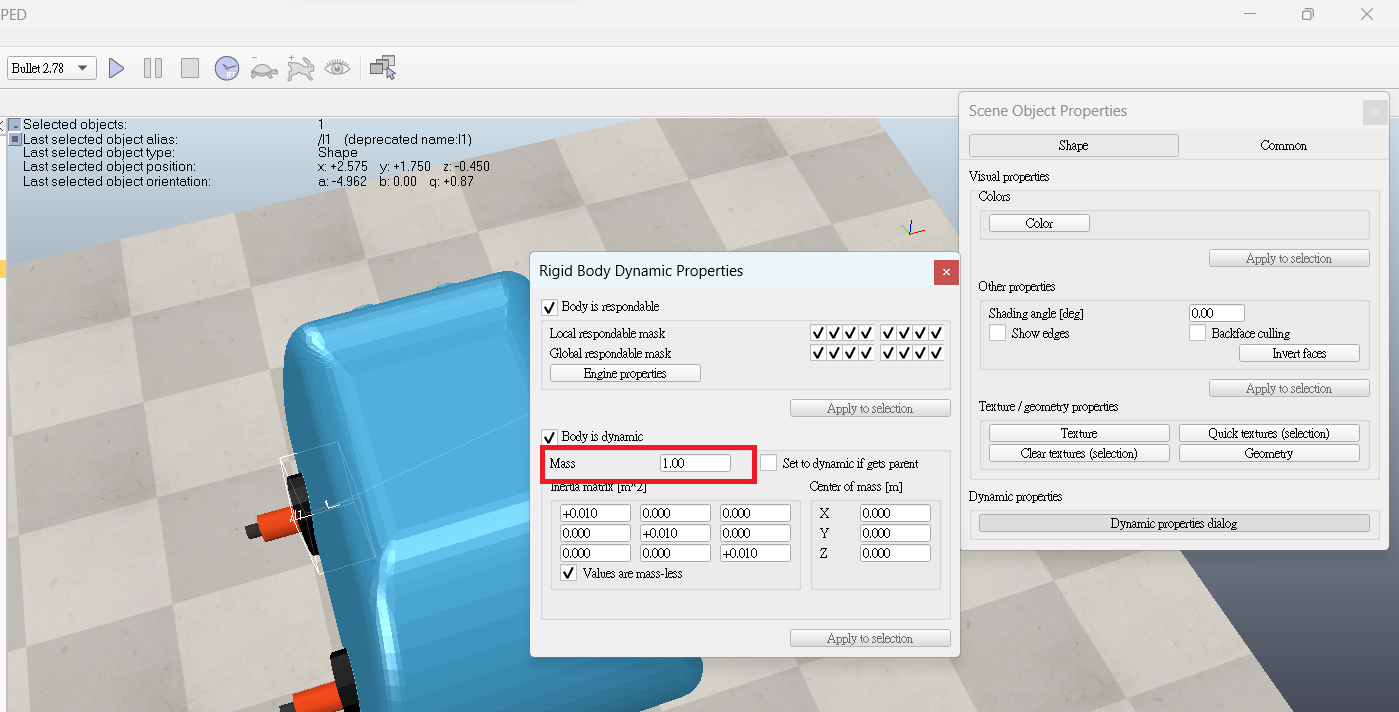
\includegraphics[width=0.5\textwidth]{球員組裝_10.png}
  \end{center}
  \caption{調整物件質量參數}
  \label{fig:photo}
\end{figure}
\newpage

\section{背號}
\begin{figure}[h]
  \begin{center}
    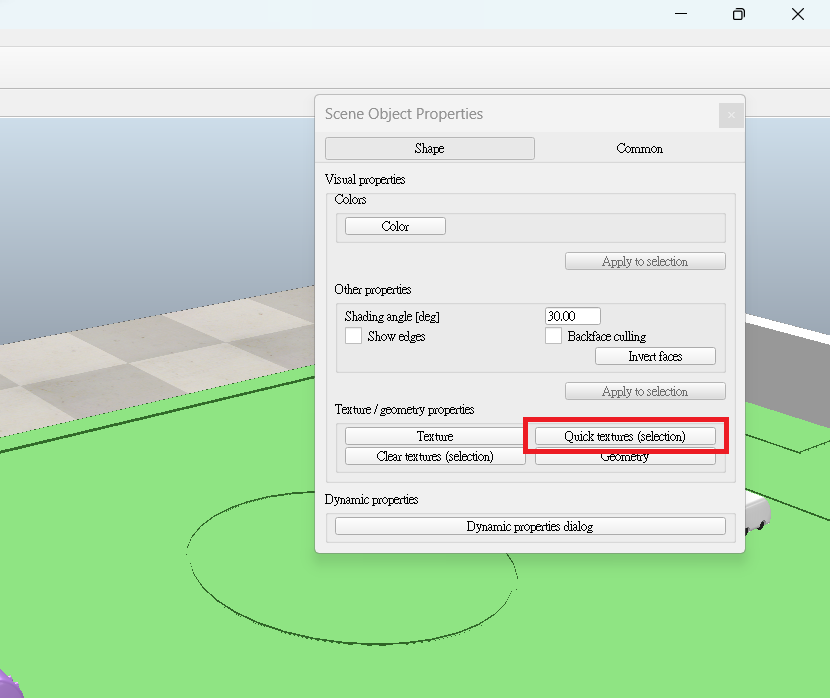
\includegraphics[width=0.5\textwidth]{球員背號_1.png}
  \end{center}
  \caption{變更物件材質(將數字貼在物件上)}
  \label{fig:photo}
\end{figure}
\begin{figure}[h]
  \begin{center}
    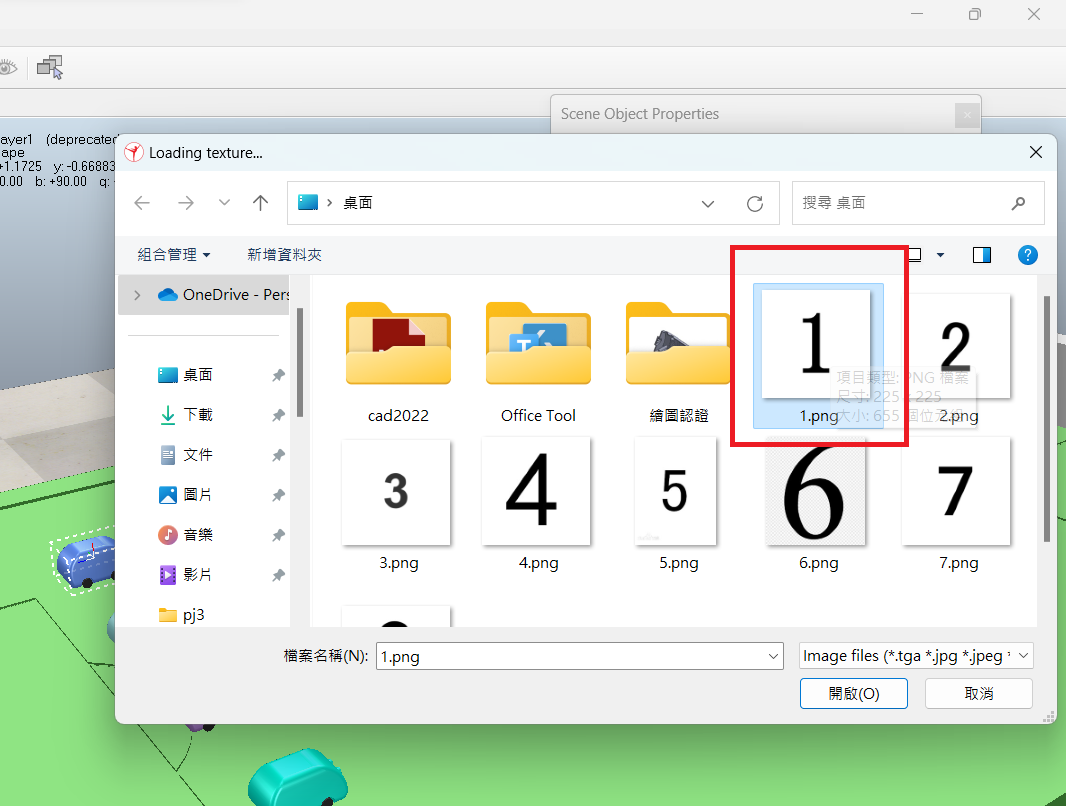
\includegraphics[width=0.5\textwidth]{球員背號_2.png}
  \end{center}
  \caption{選擇要使用的圖案}
  \label{fig:photo}
\end{figure}
\begin{figure}[h]
  \begin{center}
    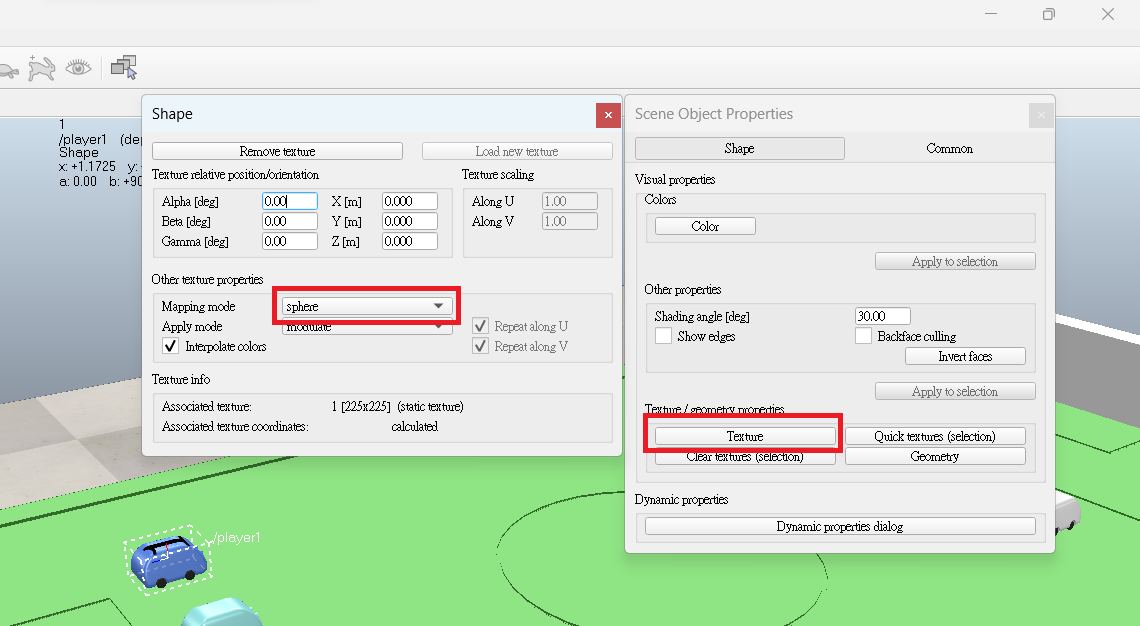
\includegraphics[width=0.5\textwidth]{球員背號_3.png}
  \end{center}
  \caption{調整映像參數}
  \label{fig:photo}
\end{figure}
\begin{figure}[h]
  \begin{center}
    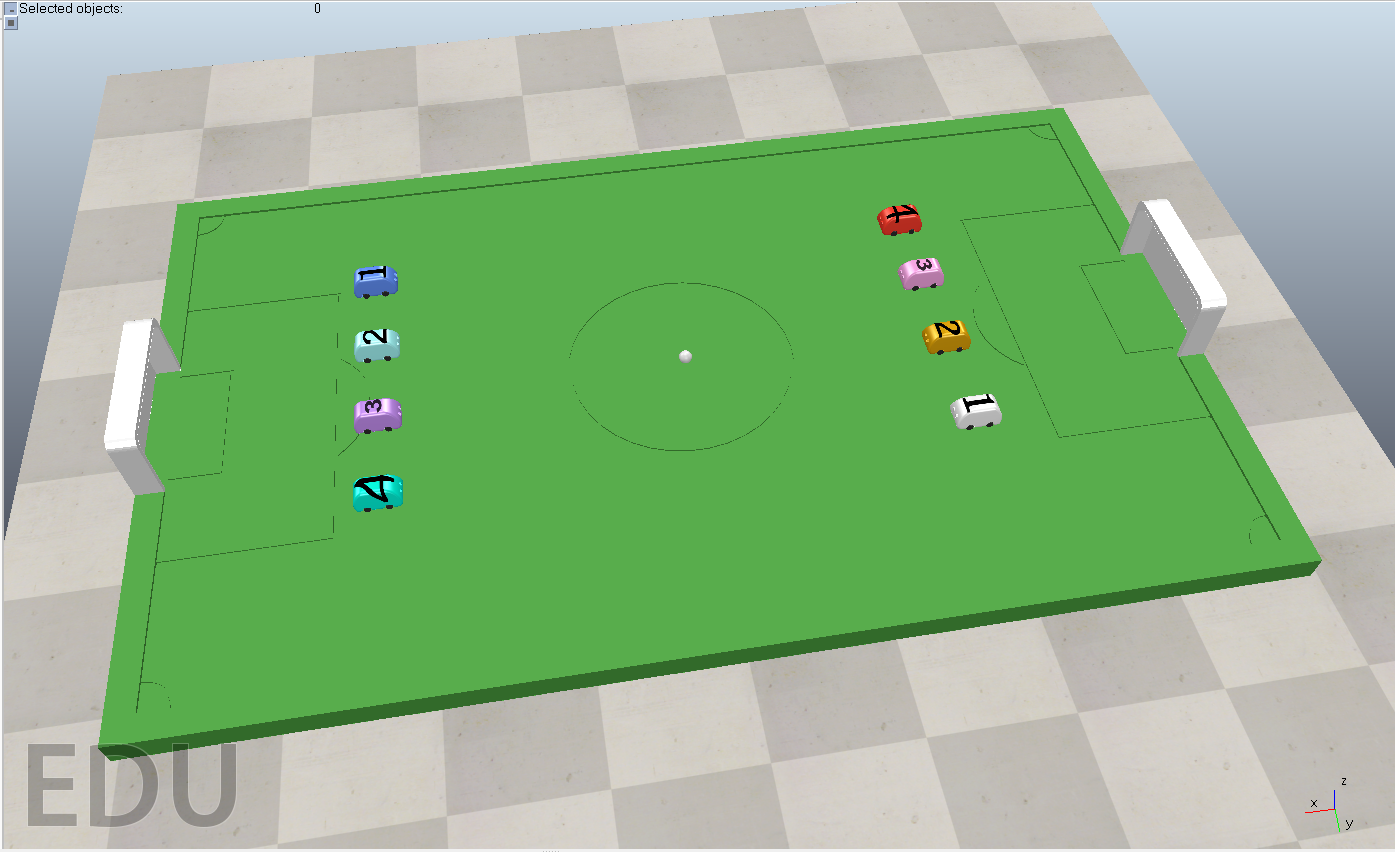
\includegraphics[width=0.5\textwidth]{球員背號_4.png}
  \end{center}
  \caption{背號完成}
  \label{fig:photo}
\end{figure}
\newpage

\section{程式碼}
連線主機---使用遠端 API 來連接到位於本地主機 (localhost) 上執行,RemoteAPIClient 是用於建立與遠端應用程式之間的通訊連接。指定了要連接的主機名稱為 "localhost" ,連接埠為 23000。使用 client.getObject("sim") 來獲取遠端應用程式中的一個名為 "sim" 的物件。 "Program started" 表示程式開始執行,然後程式執行 client.getObject("sim") 這行程式碼後,輸出了 "Simulation started" ,表示模擬 (simulation) 開始執行。
\begin{lstlisting}[language=Python, frame=single, numbers=left, captionpos=b, basicstyle=\ttfamily\small,showstringspaces=false, breaklines=true, tabsize=4, xleftmargin=15pt]
client = RemoteAPIClient('localhost', 23000)
print('Program started')
sim = client.getObject('sim')
#sim.startSimulation()
print('Simulation started')
\end{lstlisting}

輪子速度---定義一個 setBubbleRobVelocity 的函式,用於設定 BubbleRob 模型的輪子速度。首先使用 sim.getObject 函式獲取四個物件 leftMotor1、rightMotor1、leftMotor2、rightMotor2。用 sim.setJointTargetVelocity 函式 >>>設定輪子的目標速度,setJointTargetVelocity 函式 >>>設定 joint 的目標速度,因此可以用來控制輪子的運動。函式中的四個參數 leftWheelVelocity1、rightWheelVelocity1、leftWheelVelocity2、rightWheelVelocity2 分別代表四個輪子的速度。這些參數將會被傳遞給對應的 setJointTargetVelocity 函式來設定輪子的目標速度。
\begin{lstlisting}[language=Python, frame=single, numbers=left, captionpos=b, basicstyle=\ttfamily\small,showstringspaces=false, breaklines=true, tabsize=4, xleftmargin=15pt]
def setBubbleRobVelocity(leftWheelVelocity1, rightWheelVelocity1,leftWheelVelocity2, rightWheelVelocity2):
    leftMotor1 = sim.getObject('/lM1')
    rightMotor1 = sim.getObject('/rM1')
    leftMotor2 = sim.getObject('/lM2')
    rightMotor2 = sim.getObject('/rM2')
    sim.setJointTargetVelocity(leftMotor1, leftWheelVelocity1)
    sim.setJointTargetVelocity(rightMotor1, rightWheelVelocity1)
    sim.setJointTargetVelocity(leftMotor2, leftWheelVelocity2)
    sim.setJointTargetVelocity(rightMotor2, rightWheelVelocity2)
    #輸入四個變數分別給四個軸速度
\end{lstlisting}

輪子方向---定義名為 setBubbleRobangel 的函式。目的是根據輸入的參數 a,改變 BubbleRob 模型的前輪方向。首先使用 sim.getObject 函式獲取物件 bR,它代表 BubbleRob 模型的身體 (body)。接著程式計算出一個 angel 列表。angel 列表包含三個元素,第一個元素為 -90 度轉換為弳度的值,第二個元素為 a 度轉換為弳度的值,第三個元素為 0。然後用 sim.getObject 函式分別獲取物件 leftMotor 和 rightMotor,它們分別代表 BubbleRob 模型的左輪和右輪。最後使用 sim.setObjectOrientation 函式來設定物件的方向。該函式用於設定物件相對於參考物件的方向。在這裡將 leftMotor 和 rightMotor 的方向設定為相對於 bR 物件的方向,方向由 angel 列表指定。
\begin{lstlisting}[language=Python, frame=single, numbers=left, captionpos=b, basicstyle=\ttfamily\small,showstringspaces=false, breaklines=true, tabsize=4, xleftmargin=15pt]
def setBubbleRobangel(a):
    bR = sim.getObject('/bR')
    angel = [-90*math.pi/180, a*math.pi/180, 0]
    leftMotor = sim.getObject('/lM1')
    rightMotor = sim.getObject('/rM1')
    sim.setObjectOrientation(leftMotor, bR, angel)
    sim.setObjectOrientation(rightMotor, bR, angel)
    #輸入一個變數改變前輪方向
\end{lstlisting}

控制---這段程式碼是一個無窮迴圈,它會持續監聽鍵盤的按鍵輸入,並根據按下的按鍵來控制 BubbleRob 模型的運動。目的是根據鍵盤輸入來控制 BubbleRob 模型的運動,並提供了前進、後退、旋轉和停止等功能。程式碼中使用 "keyboard.is_pressed" 函式來判斷指定的按鍵是否被按下。 |若按下 'w' 鍵,則呼叫 "setBubbleRobVelocity(4, 4, 4, 4)" 來設定 BubbleRob 模型的速度為正向,並根據 'a' 和 'd' 鍵的狀態設定前輪的方向。 |若按下 's' 鍵,則呼叫 "setBubbleRobVelocity(-4, -4, -4, -4)" 來設定 BubbleRob 模型的速度為負向,並根據 'a' 和 'd' 鍵的狀態設定前輪的方向。 |若按下 'a' 鍵,則呼叫 "setBubbleRobVelocity(-4, 4, -4, 4)" 來設定 BubbleRob 模型的速度使其向左旋轉。 |若按下 'd' 鍵,則呼叫 "setBubbleRobVelocity(4, -4, 4, -4)" 來設定 BubbleRob 模型的速度使其向右旋轉。 |若按下 'q' 鍵,則停止模擬 (simulation)。 |若沒有按下任何按鍵,則呼叫 "setBubbleRobVelocity(0, 0, 0, 0)" 和 "setBubbleRobangel(0)",將 BubbleRob 模型的速度和前輪方向設定為零,即停止移動。
\begin{lstlisting}[language=Python, frame=single, numbers=left, captionpos=b, basicstyle=\ttfamily\small,showstringspaces=false, breaklines=true, tabsize=4, xleftmargin=15pt]
while True:
    if keyboard.is_pressed('w'):
        setBubbleRobVelocity(4, 4, 4, 4)
        if keyboard.is_pressed('a'):
            setBubbleRobangel(-40)
        elif keyboard.is_pressed('d'):
            setBubbleRobangel(40)
        else:
            setBubbleRobangel(0)
    elif keyboard.is_pressed('s'):
        setBubbleRobVelocity(-4, -4, -4, -4)
        if keyboard.is_pressed('a'):
            setBubbleRobangel(-40)
        elif keyboard.is_pressed('d'):
            setBubbleRobangel(40)
        else:
            setBubbleRobangel(0)
    elif keyboard.is_pressed('a'):
        setBubbleRobVelocity(-4, 4, -4, 4)
    elif keyboard.is_pressed('d'):
        setBubbleRobVelocity(4, -4, 4, -4)
    elif keyboard.is_pressed('q'):
        % stop simulation
        sim.stopSimulation()
    else:
        setBubbleRobVelocity(0, 0, 0, 0)
        setBubbleRobangel(0)
\end{lstlisting}
\newpage

\chapter{記分板}
\section{繪圖}
\begin{figure}[hbt!]
  \centering
  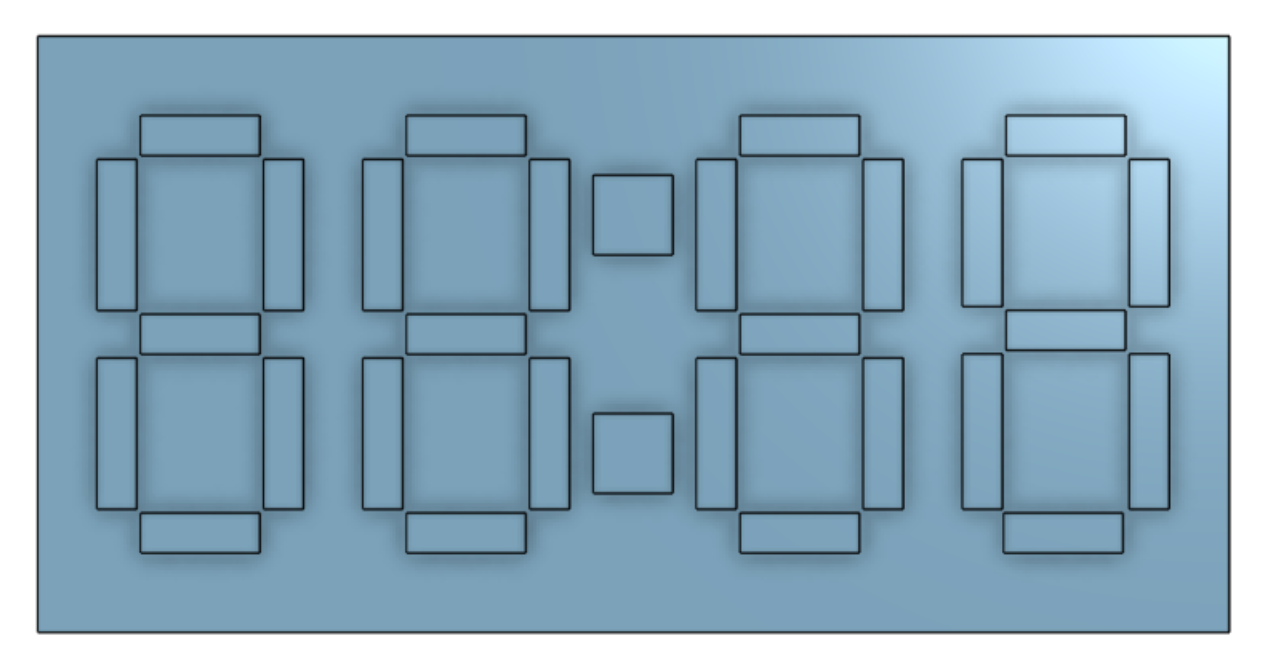
\includegraphics[width=0.5\textwidth]{計分板繪圖_17.png}
\end{figure}
\begin{figure}[hbt!]
  \centering
  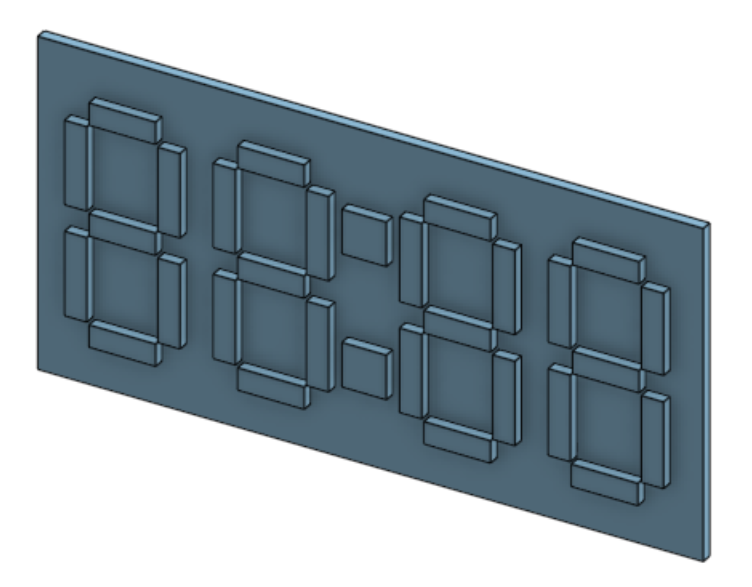
\includegraphics[width=0.5\textwidth]{計分板繪圖_18.png}
  \caption{LED記分板_1}
  \label{fig:photo1}
\end{figure}

\begin{figure}[hbt!]
  \centering
  
\includegraphics[width=0.5\textwidth]{計分板繪圖_15.png}
\end{figure}
\begin{figure}[hbt!]
  \centering
  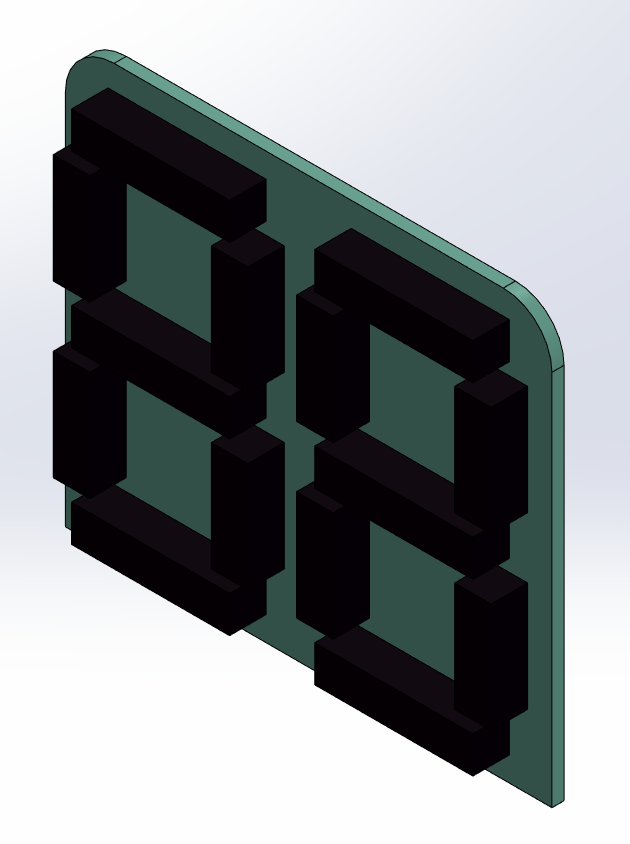
\includegraphics[width=0.5\textwidth]{計分板繪圖_16.png}
  \caption{LED記分板_2}
  \label{fig:photo2}
\end{figure}

\begin{figure}[hbt!]
  \centering
  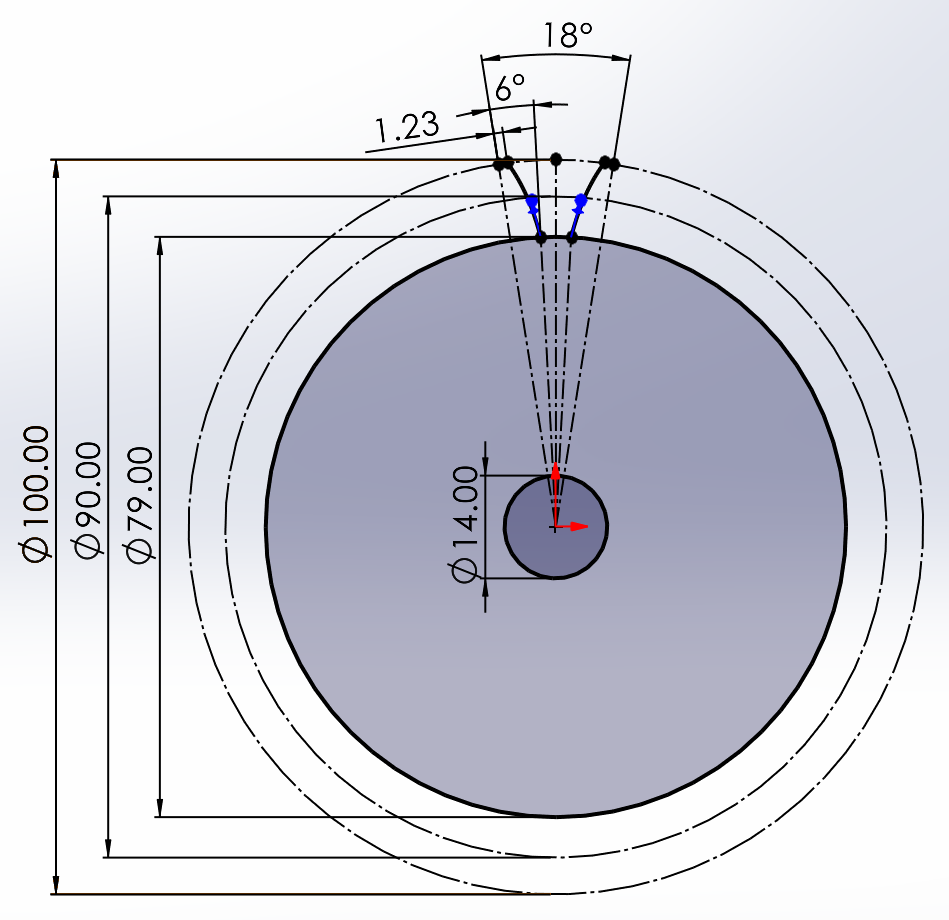
\includegraphics[width=0.5\textwidth]{計分板繪圖_1.png}
\end{figure}
\begin{figure}[hbt!]
  \centering
  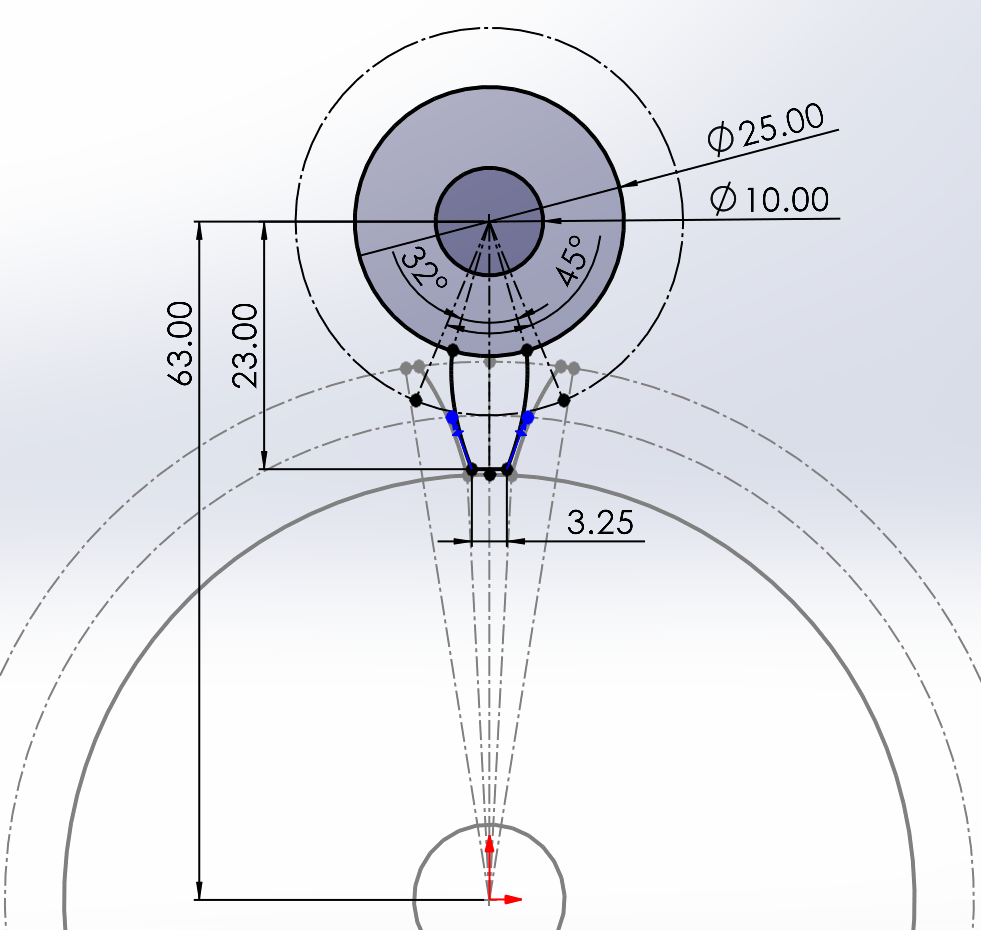
\includegraphics[width=0.5\textwidth]{計分板繪圖_2.png}
  \caption{sketch}
  \label{fig:photo3}
\end{figure}

\begin{figure}[hbt!]
  \centering
  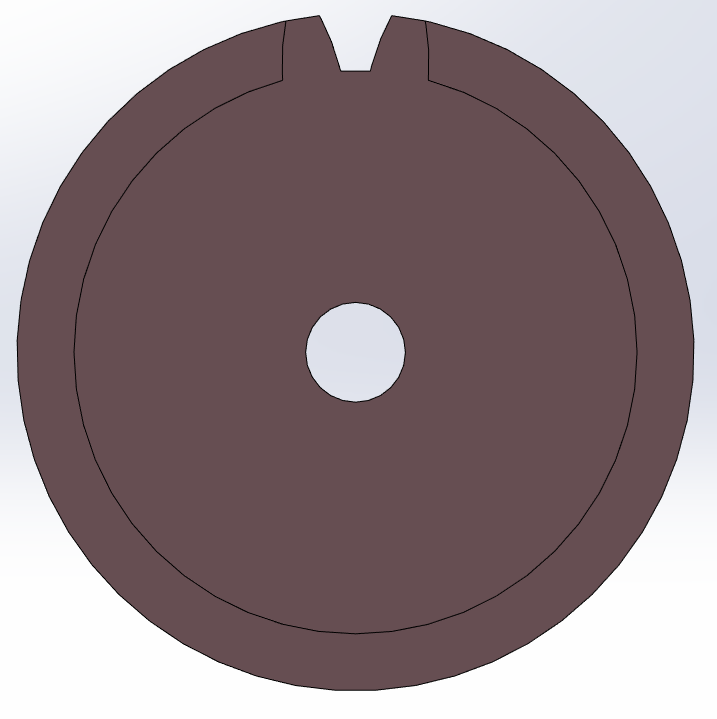
\includegraphics[width=0.5\textwidth]{計分板繪圖_3.png}
\end{figure}
\begin{figure}[hbt!]
  \centering
  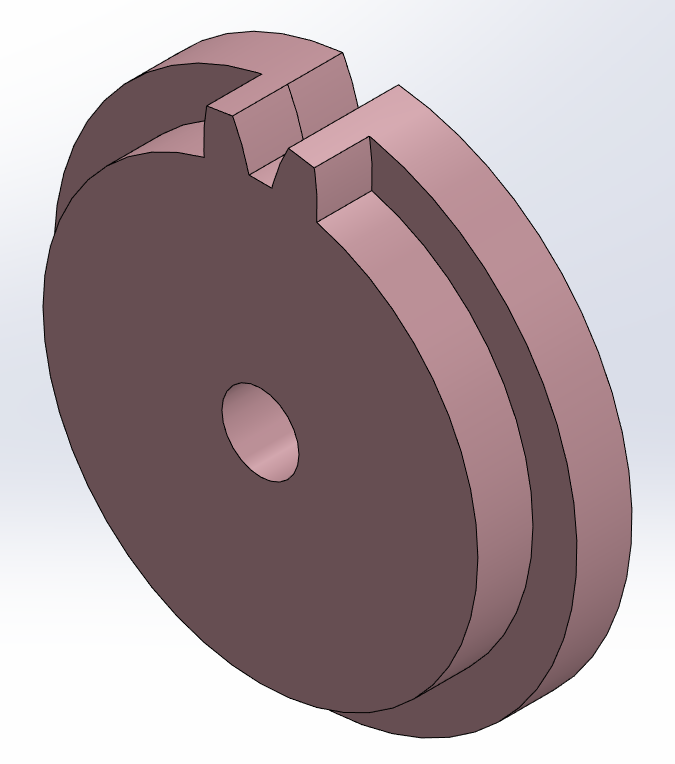
\includegraphics[width=0.5\textwidth]{計分板繪圖_4.png}
  \caption{Advancing Wheel gear}
  \label{fig:photo4}
\end{figure}

\begin{figure}[hbt!]
  \centering
  
\includegraphics[width=0.5\textwidth]{計分板繪圖_5.png}
\end{figure}
\begin{figure}[hbt!]
  \centering
  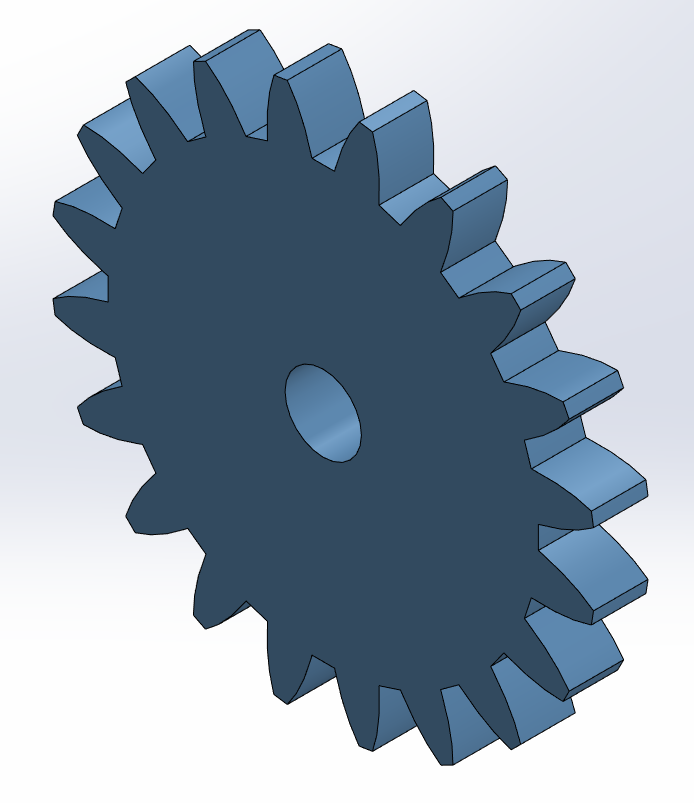
\includegraphics[width=0.5\textwidth]{計分板繪圖_6.png}
  \caption{M4.5 Teeth20 gear}
  \label{fig:photo5}
\end{figure}

\begin{figure}[hbt!]
  \centering
  
\includegraphics[width=0.5\textwidth]{計分板繪圖_7.png}
\end{figure}
\begin{figure}[hbt!]
  \centering
  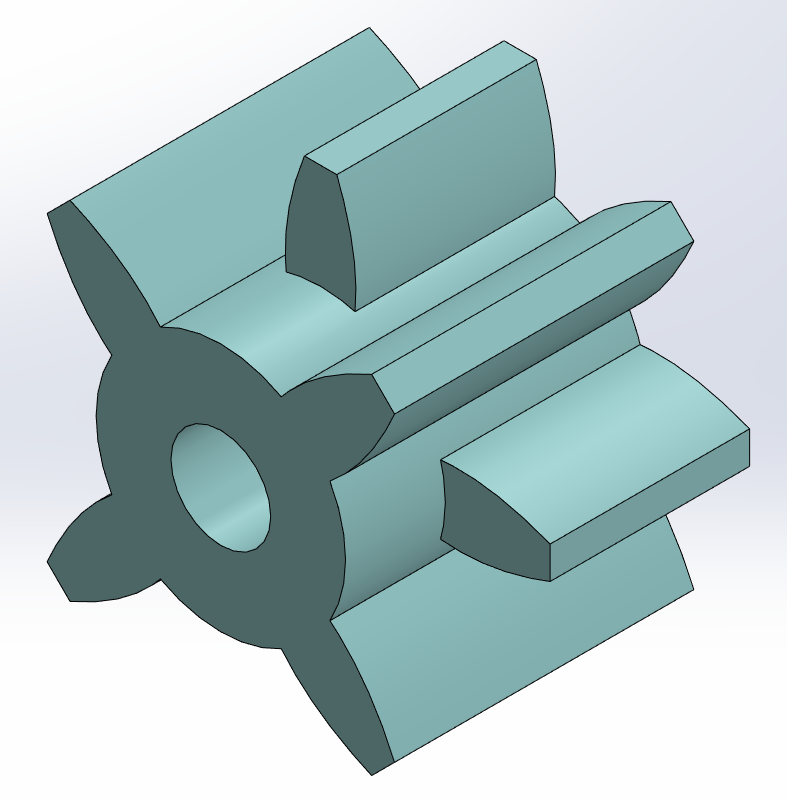
\includegraphics[width=0.5\textwidth]{計分板繪圖_8.png}
  \caption{M4.5 Teeth8 gear}
  \label{fig:photo6}
\end{figure}

\begin{figure}[hbt!]
  \centering
  
\includegraphics[width=0.5\textwidth]{計分板繪圖_11.png}
\end{figure}
\begin{figure}[hbt!]
  \centering
  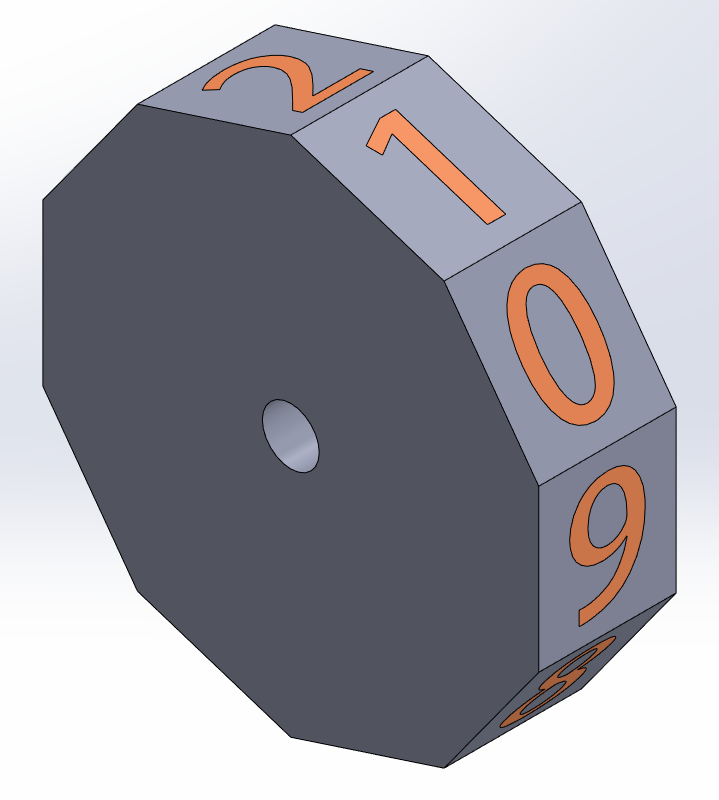
\includegraphics[width=0.5\textwidth]{計分板繪圖_12.png}
  \caption{Number Wheel}
  \label{fig:photo7}
\end{figure}

\begin{figure}[hbt!]
  \centering
  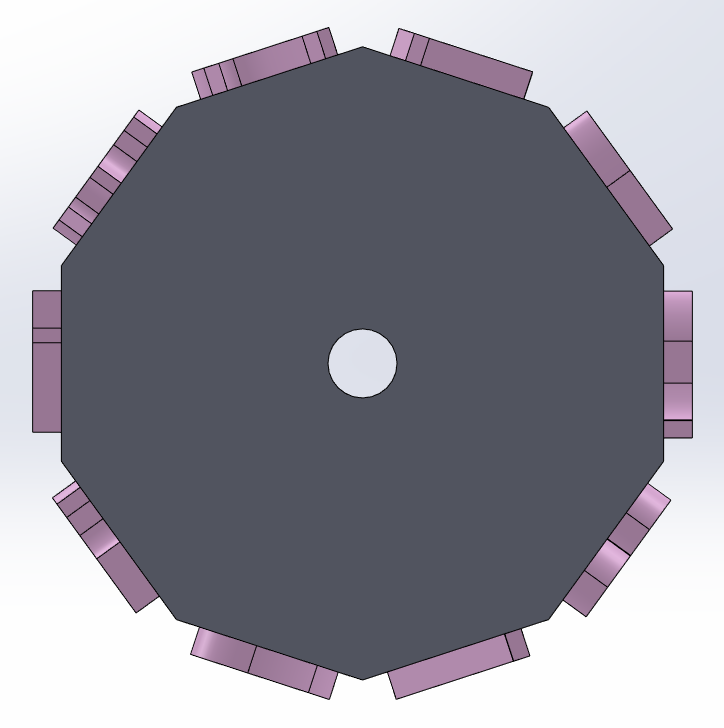
\includegraphics[width=0.5\textwidth]{計分板繪圖_9.png}
\end{figure}
\begin{figure}[hbt!]
  \centering
  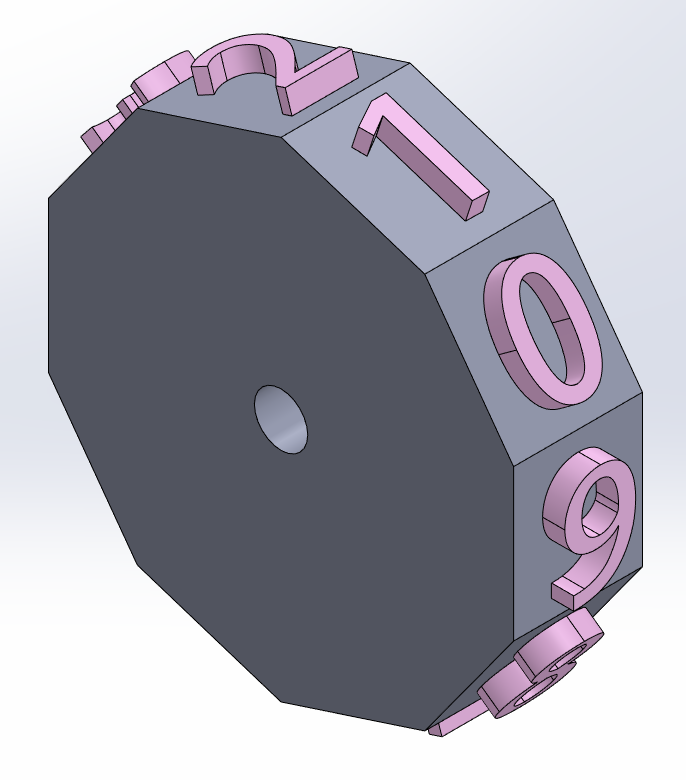
\includegraphics[width=0.5\textwidth]{計分板繪圖_10.png}
  \caption{Number Wheel1}
  \label{fig:photo8}
\end{figure}

\begin{figure}[hbt!]
  \centering
  
\includegraphics[width=0.5\textwidth]{計分板繪圖_13.png}
\end{figure}
\begin{figure}[hbt!]
  \centering
  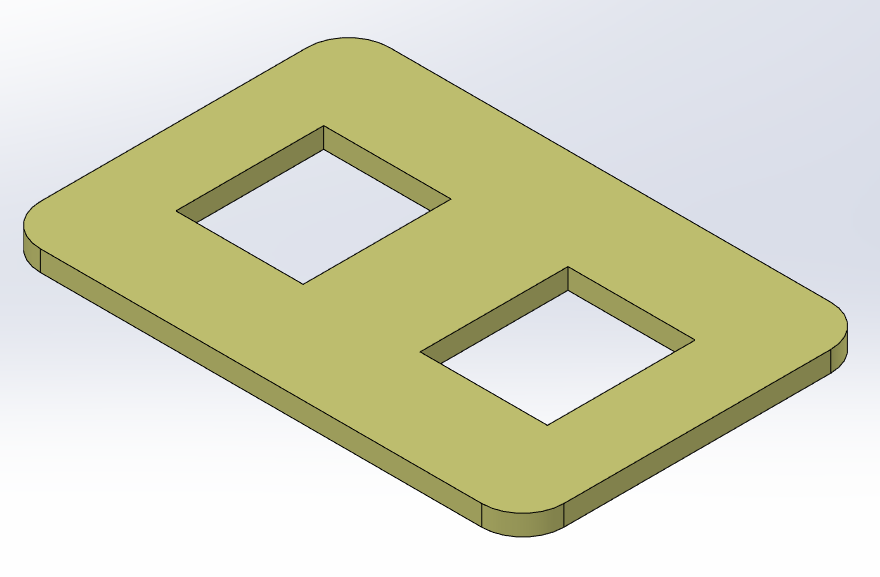
\includegraphics[width=0.5\textwidth]{計分板繪圖_14.png}
  \caption{board}
  \label{fig:photo9}
\end{figure}

\section{組合}
\begin{figure}[hbt!]
  \centering
  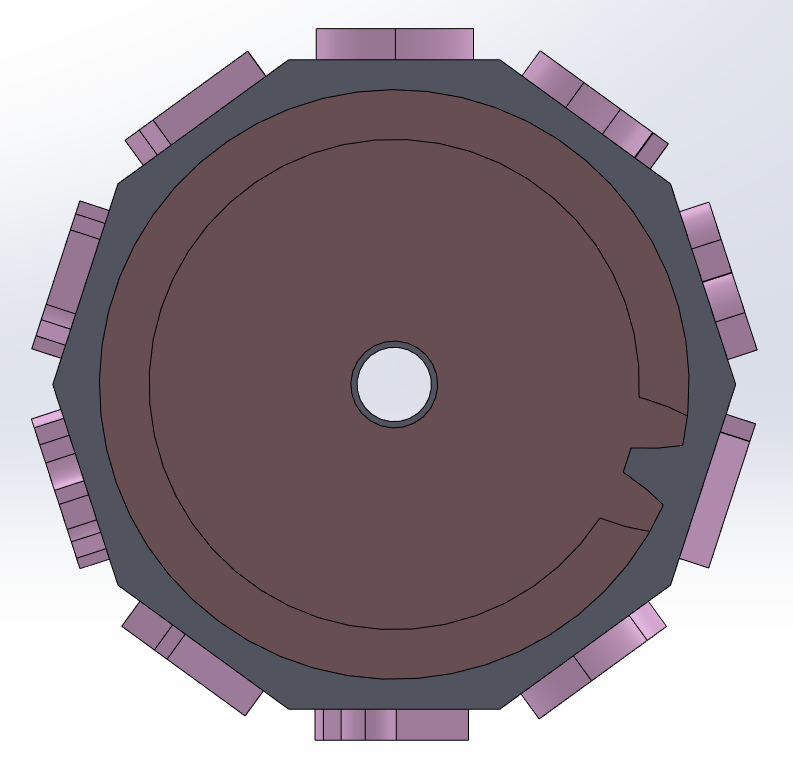
\includegraphics[width=0.5\textwidth]{計分板組合_1.png}
\end{figure}
\begin{figure}[hbt!]
  \centering
  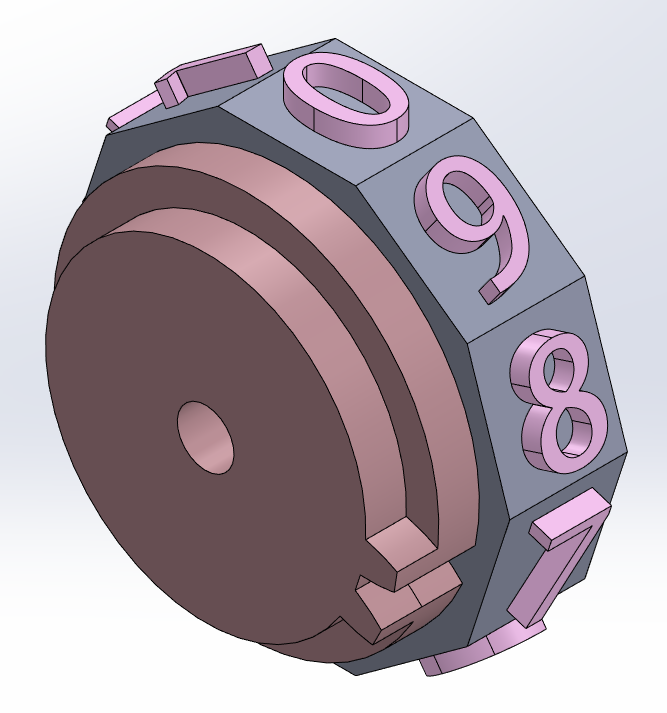
\includegraphics[width=0.5\textwidth]{計分板組合_2.png}
  \caption{Unit Digit Wheel}
  \label{fig:photo10}
\end{figure}

\begin{figure}[hbt!]
  \centering
  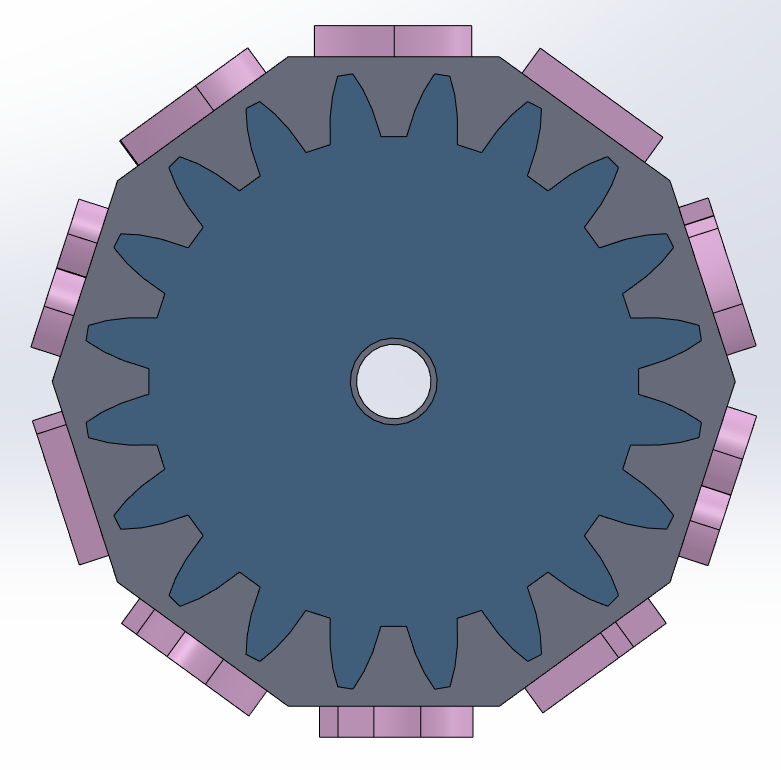
\includegraphics[width=0.5\textwidth]{計分板組合_3.png}
\end{figure}
\begin{figure}[hbt!]
  \centering
  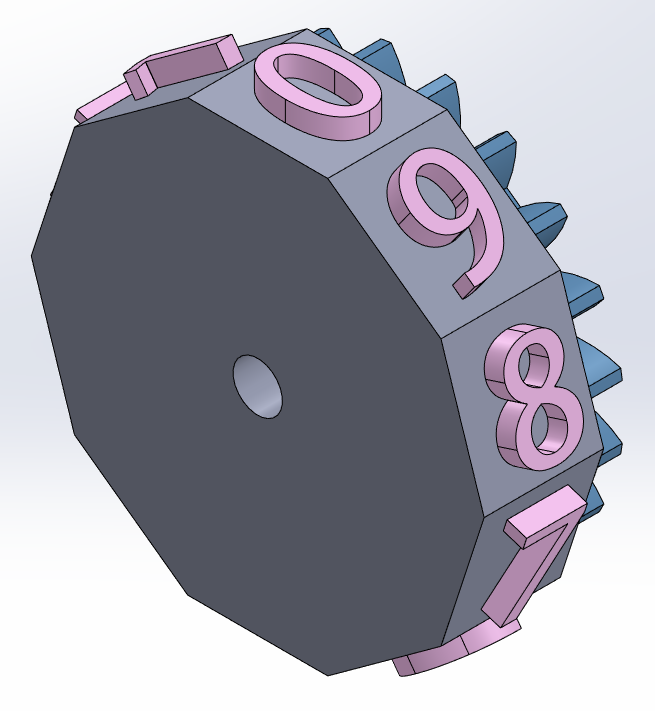
\includegraphics[width=0.5\textwidth]{計分板組合_4.png}
  \caption{Ten's Digit Wheel}
  \label{fig:photo11}
\end{figure}

\begin{figure}[hbt!]
  \centering
  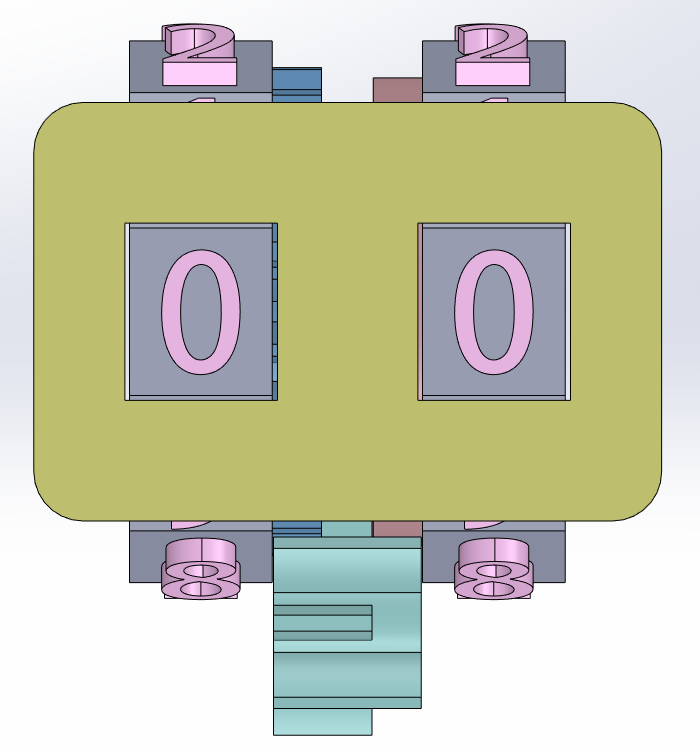
\includegraphics[width=0.5\textwidth]{計分板組合_5.png}
\end{figure}
\begin{figure}[hbt!]
  \centering
  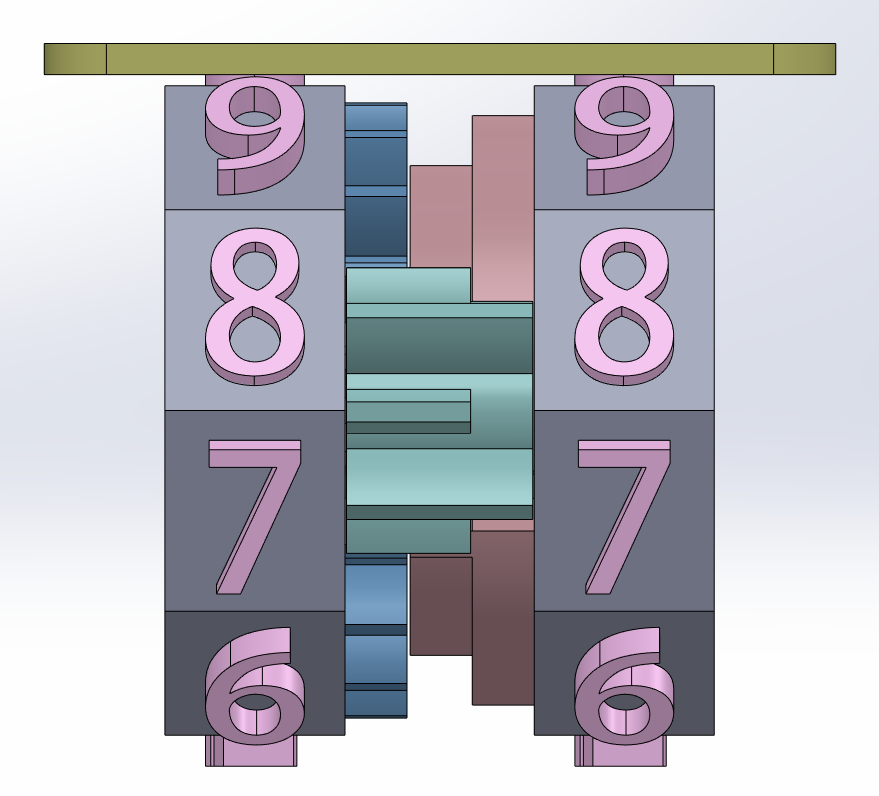
\includegraphics[width=0.5\textwidth]{計分板組合_6.png}
\end{figure}
\begin{figure}[hbt!]
  \centering
  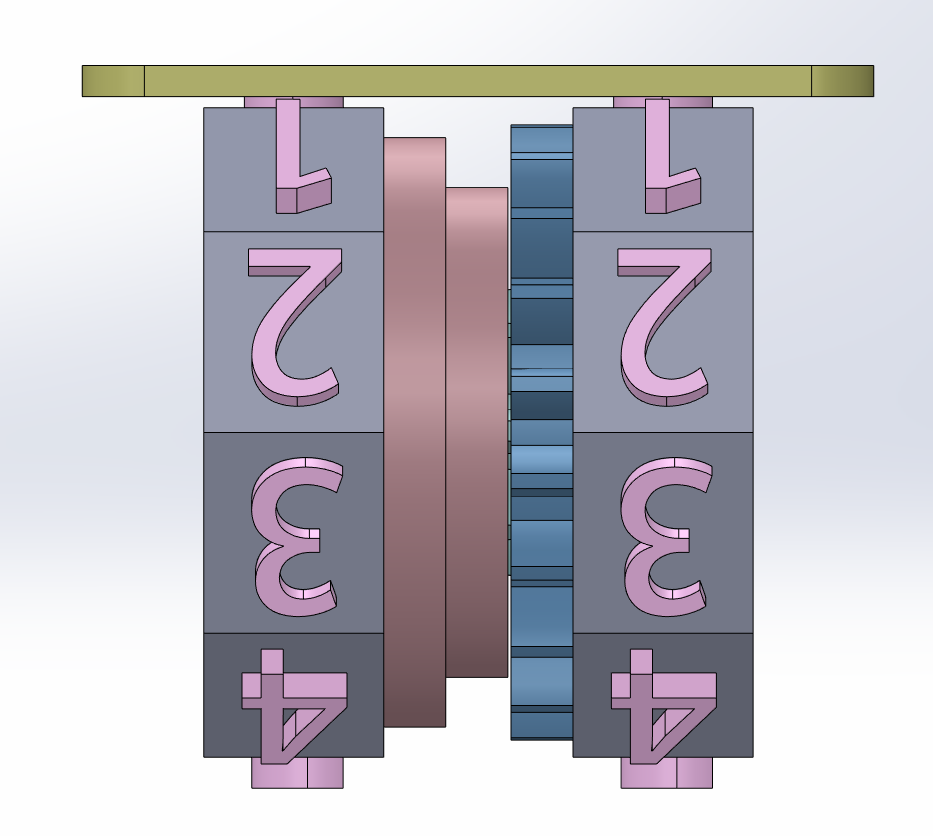
\includegraphics[width=0.5\textwidth]{計分板組合_7.png}
\end{figure}
\begin{figure}[hbt!]
  \centering
  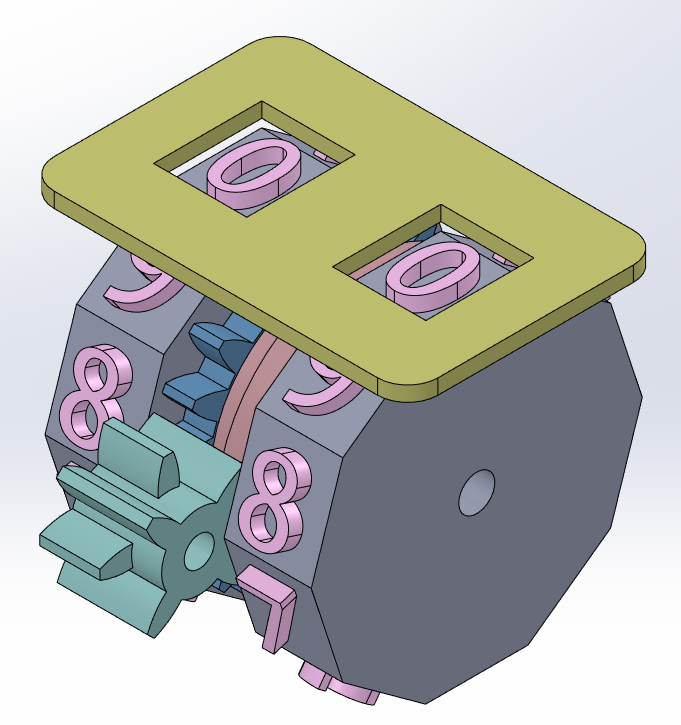
\includegraphics[width=0.5\textwidth]{計分板組合_8.png}
  \caption{Mechanical Counter}
  \label{fig:photo12}
\end{figure}

\section{組裝}
\begin{figure}[hbt!]
  \centering
  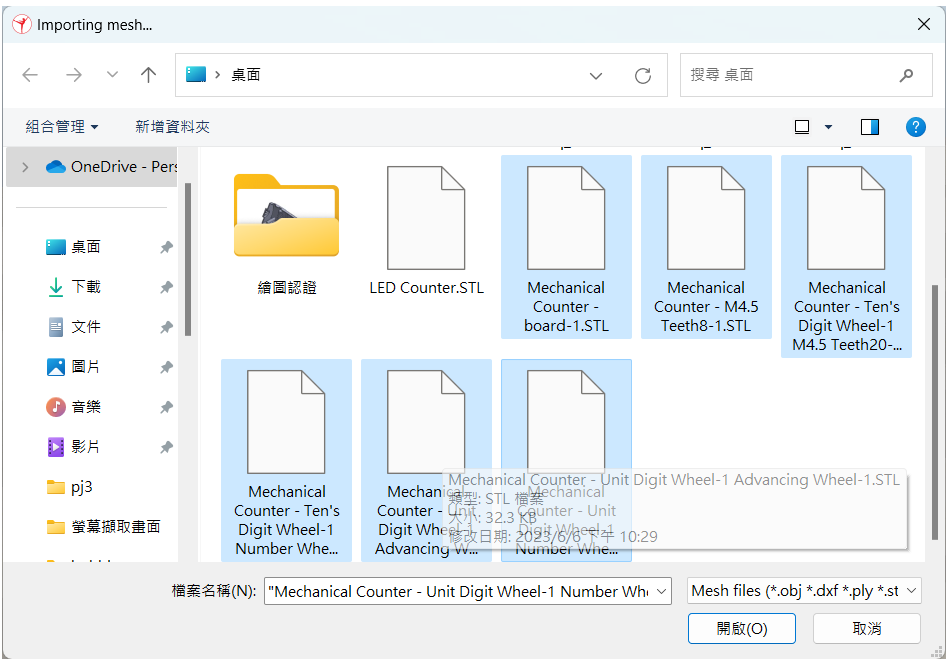
\includegraphics[width=0.5\textwidth]{記分板組裝_1.png}
\end{figure}
\begin{figure}[hbt!]
  \centering
  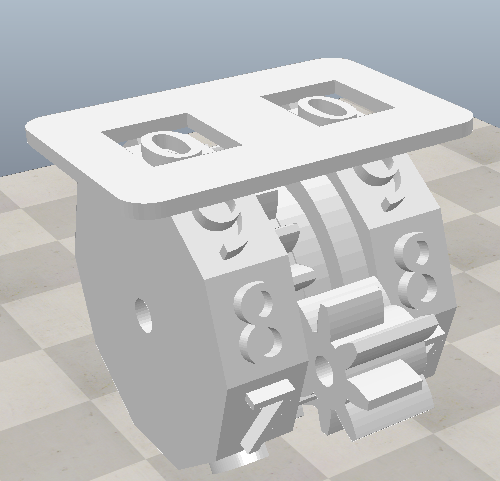
\includegraphics[width=0.5\textwidth]{記分板組裝_2.png}
  \caption{一次選取所有STL檔導入}
  \label{fig:photo13}
\end{figure}

\begin{figure}[hbt!]
  \begin{center}
    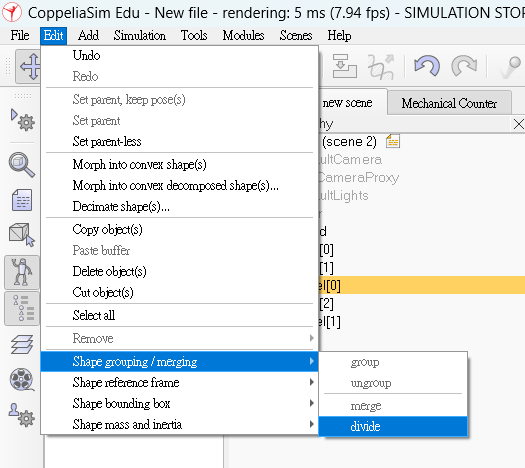
\includegraphics[width=0.5\textwidth]{記分板組裝_3.png}
  \end{center}
  \caption{將wheel物件爆炸分解}
  \label{fig:photo}
\end{figure}

\begin{figure}[hbt!]
  \begin{center}
    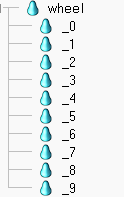
\includegraphics[width=0.5\textwidth]{記分板組裝_4.png}
  \end{center}
  \caption{更改數字名稱}
  \label{fig:photo}
\end{figure}

\begin{figure}[hbt!]
  \begin{center}
    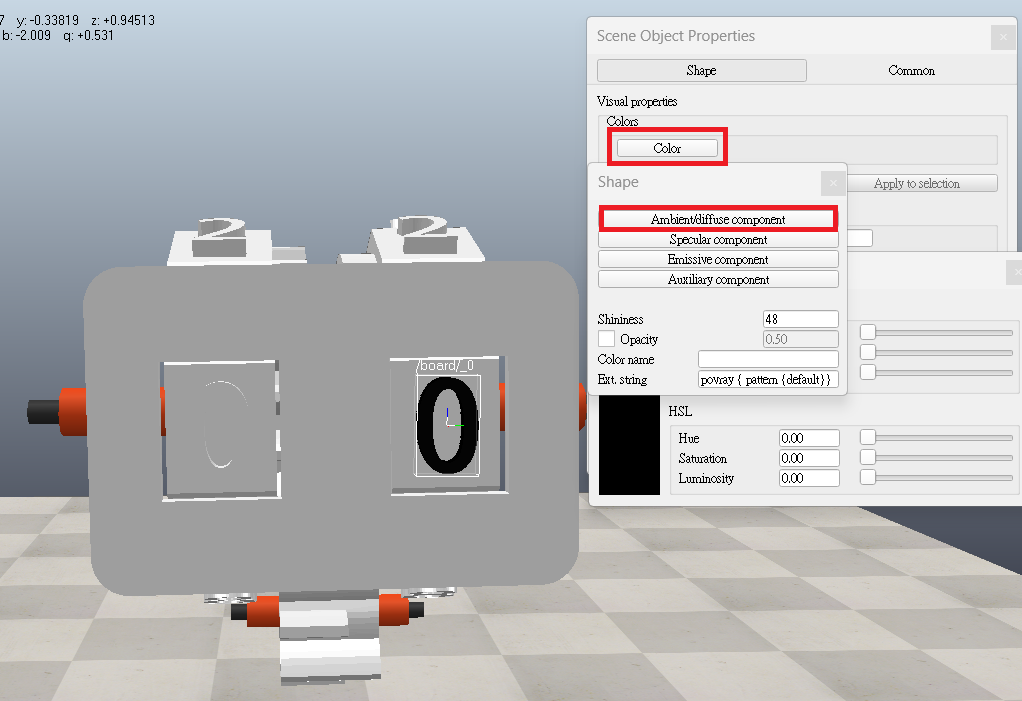
\includegraphics[width=0.5\textwidth]{記分板組裝_5.png}
  \end{center}
  \caption{更改數字顏色}
  \label{fig:photo}
\end{figure}

\begin{figure}[hbt!]
  \begin{center}
    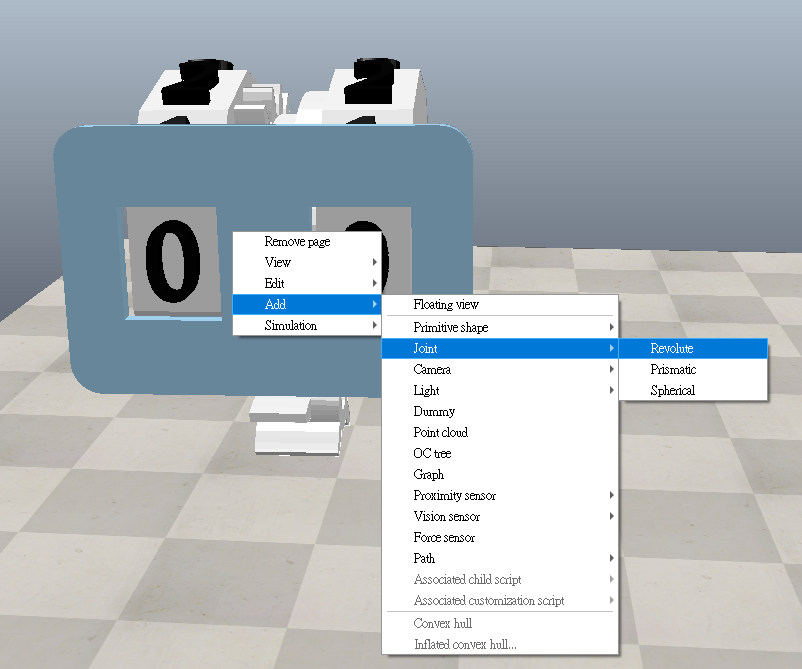
\includegraphics[width=0.5\textwidth]{記分板組裝_8.png}
  \end{center}
  \caption{新增Joint}
  \label{fig:photo}
\end{figure}

\begin{figure}[hbt!]
  \begin{center}
    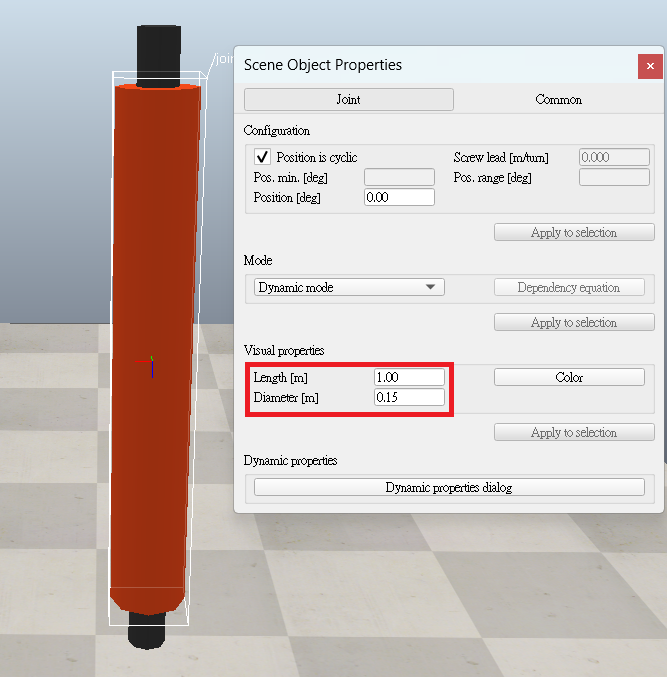
\includegraphics[width=0.5\textwidth]{記分板組裝_9.png}
  \end{center}
  \caption{調整Joint方向及大小}
  \label{fig:photo}
\end{figure}

\begin{figure}[hbt!]
  \begin{center}
    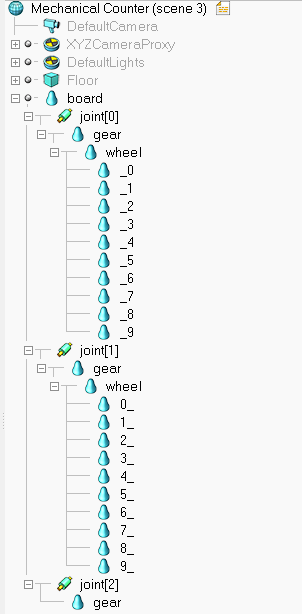
\includegraphics[width=0.5\textwidth]{記分板組裝_7.png}
  \end{center}
  \caption{物件相互依附}
  \label{fig:photo}
\end{figure}

\begin{figure}[hbt!]
  \begin{center}
    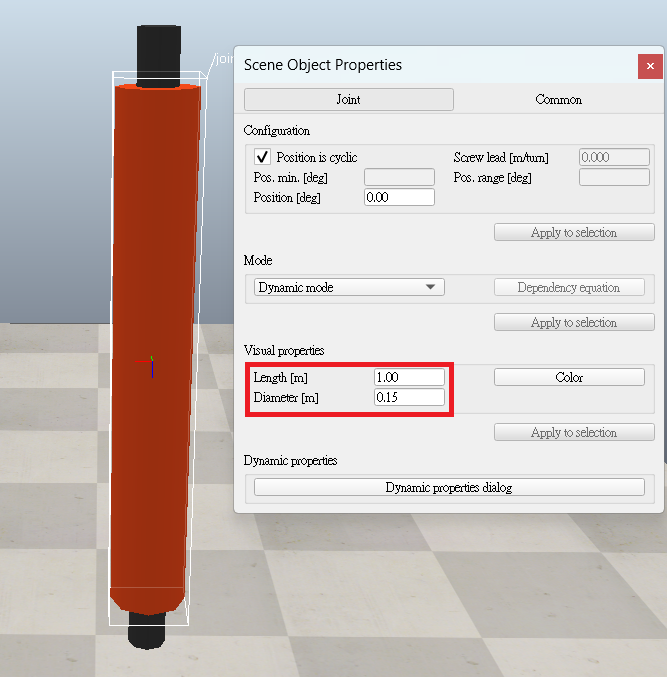
\includegraphics[width=0.5\textwidth]{記分板組裝_9.png}
  \end{center}
  \caption{調整Joint方向及大小}
  \label{fig:photo}
\end{figure}

\begin{figure}[hbt!]
  \begin{center}
    \includegraphics[width=0.5\textwidth]{記分板組裝_10.png}
  \end{center}
  \caption{調整物件傳動參數}
  \label{fig:photo}
\end{figure}

\begin{figure}[hbt!]
  \begin{center}
    \includegraphics[width=0.5\textwidth]{記分板組裝_11.png}
  \end{center}
  \caption{調整物件質量參數}
  \label{fig:photo}
\end{figure}

\begin{figure}[hbt!]
  \begin{center}
    \includegraphics[width=0.5\textwidth]{記分板組裝_12.png}
  \end{center}
  \caption{完成記分板}
  \label{fig:photo}
\end{figure}

\chapter{場景}
\section{匯入球場 球門 球員 記分板}
\begin{figure}[hbt!]
  \begin{center}
    \includegraphics[width=1\textwidth]{場景.png}
  \end{center}
  \caption{Scene}
  \label{fig:photo}
\end{figure}

\chapter{跨網路連線}
\section{設定連線步驟}
\begin{figure}[hbt!]
  \begin{center}
    \includegraphics[width=0.5\textwidth]{連線_1.png}
  \end{center}
  \caption[關閉防火牆]{\phantomsection}
  \label{fig:photo}
\end{figure}

\begin{figure}[hbt!]
  \begin{center}
    \includegraphics[width=0.5\textwidth]{連線_2.png}
  \end{center}
  \caption[點選進階設定]{\phantomsection}
  \label{fig:photo}
\end{figure}

\begin{figure}[hbt!]
  \begin{center}
    \includegraphics[width=0.5\textwidth]{連線_3.png}
  \end{center}
  \caption[設定輸入及輸出規則類型]{\phantomsection}
  \label{fig:photo}
\end{figure}

\begin{figure}[hbt!]
  \begin{center}
    \includegraphics[width=0.5\textwidth]{連線_4.png}
  \end{center}
  \caption[設定特定遠端連接埠]{\phantomsection}
  \label{fig:photo}
\end{figure}

\begin{figure}[hbt!]
  \begin{center}
    \includegraphics[width=0.5\textwidth]{連線_5.png}
  \end{center}
  \caption[v允許連線]{\phantomsection}
  \label{fig:photo}
\end{figure}

\begin{figure}[hbt!]
  \begin{center}
    \includegraphics[width=0.5\textwidth]{連線_6.png}
  \end{center}
  \caption[設定名稱]{\phantomsection}
  \label{fig:photo}
\end{figure}

\begin{figure}[hbt!]
  \begin{center}
    \includegraphics[width=0.5\textwidth]{連線_7.png}
  \end{center}
  \caption[設定規定的ipv6]{\phantomsection}
  \label{fig:photo}
\end{figure}

\newpage

\section{程式碼}
\begin{lstlisting}[language=Python, frame=single, numbers=left, captionpos=b, basicstyle=\ttfamily\small,showstringspaces=false, breaklines=true, tabsize=4, xleftmargin=15pt]
# pip install pyzmq cbor keyboard
from zmqRemoteApi import RemoteAPIClient
import keyboard

client = RemoteAPIClient('localhost', 23000)

print('Program started')
sim = client.getObject('sim')

sim.startSimulation()
print('Simulation started')

def setBubbleRobVelocity(leftWheelVelocity, rightWheelVelocity):
    leftMotor = sim.getObject('/leftMotor')
    rightMotor = sim.getObject('/rightMotor')
    sim.setJointTargetVelocity(leftMotor, leftWheelVelocity)
    sim.setJointTargetVelocity(rightMotor, rightWheelVelocity)

'''
# Example usage 1:
setBubbleRobVelocity(1.0, 1.0)
time.sleep(2)
setBubbleRobVelocity(0.0, 0.0)
'''
# use keyborad to move BubbleRob

while True:
    if keyboard.is_pressed('w'):
        setBubbleRobVelocity(1.0, 1.0)
    elif keyboard.is_pressed('s'):
        setBubbleRobVelocity(-1.0, -1.0)
    elif keyboard.is_pressed('a'):
        setBubbleRobVelocity(-1.0, 1.0)
    elif keyboard.is_pressed('d'):
        setBubbleRobVelocity(1.0, -1.0)
    elif keyboard.is_pressed('q'):
        # stop simulation
        sim.stopSimulation()
    else:
        setBubbleRobVelocity(0.0, 0.0)
\end{lstlisting}

%=---------------------相關資料----------------------=%
%\addcontentsline{toc}{chapter}{參考文獻} %新增目錄名稱
\newpage
\renewcommand\bibname{參~考~文~獻}
\begin{thebibliography}{99}  % 參考文獻印出之編號最寬為兩個字母寬
\bibitem 1\href{https://towardsdatascience.com/adam-latest-trends-in-deep-learning-optimization-6be9a291375c}{https://towardsdatascience.com/adam-latest-trends-in-deep-learning-optimization-6be9a291375c}
\bibitem 2\href{https://towardsdatascience.com/derivative-of-the-sigmoid-function-536880cf918e}{https://towardsdatascience.com/derivative-of-the-sigmoid-function-536880cf918e}
\bibitem 3\href{http://www.incompleteideas.net/book/RLbook2020.pdf}{http://www.incompleteideas.net/book/RLbook2020.pdf}
\bibitem 4\href{https://medium.com/change-the-world-with-technology/policy-gradient-181d43a24cf5}{https://medium.com/change-the-world-with-technology/policy-gradient-181d43a24cf5}
\bibitem 5\href{https://livebook.manning.com/book/grokking-deep-reinforcement-learning/chapter-11/v-11/38}{https://livebook.manning.com/book/grokking-deep-reinforcement-learning/chapter-11/v-11/38}
\bibitem 6\href{http://ukko.life.nctu.edu.tw/~u0517047/usage.html}{http://ukko.life.nctu.edu.tw/~u0517047/usage.html}
\bibitem 7\href{https://lilianweng.github.io/lil-log/2018/04/08/policy-gradient-algorithms.html}{https://lilianweng.github.io/lil-log/2018/04/08/policy-gradient-algorithms.html}\label{R.Policy Gradient}
\bibitem 8\href{https://uupgrade.medium.com/python-那些年我們一起玩過的遊戲-三-打磚塊-d89b648896ca}{https://uupgrade.medium.com/python-那些年我們一起玩過的遊戲-三-打磚塊-d89b648896ca}
\bibitem 9\href{https://cvfiasd.pixnet.net/blog/post/275774124-深度學習激勵函數介紹}{https://cvfiasd.pixnet.net/blog/post/275774124-深度學習激勵函數介紹}
\bibitem 0\href{https://www.coppeliarobotics.com/helpFiles/}{https://www.coppeliarobotics.com/helpFiles/}
\bibitem 1\href{https://hackernoon.com/the-reason-behind-moving-in-the-direction-opposite-to-the-gradient-f9566b95370b}{https://hackernoon.com/the-reason-behind-moving-in-the-direction-opposite-to-the-gradient-f9566b95370b}\label{OGD}
\bibitem 2\href{https://ruder.io/optimizing-gradient-descent/}{https://ruder.io/optimizing-gradient-descent/}
\label{OGD2}
\bibitem 3\href{https://reurl.cc/43XjEL}{https://zh.wikipedia.org/wiki/HSL和HSV色彩空間}
\label{RGBtoHSV}
\bibitem 4\href{https://reurl.cc/gzMm4N}{https://gist.github.com/karpathy/a4166c7fe253700972fcbc77e4ea32c5\# file-pg-pong-py}\label{R.pong1}
\bibitem 5\href{https://reurl.cc/95172Y}{https://github.com/schinger/pong\_ actor-critic/blob/master/pg-pong-ac.py}\label{R.pong1.1}
\bibitem 6\href{https://gist.github.com/etienne87/6803a65653975114e6c6f08bb25e1522}{https://gist.github.com/etienne87/6803a65653975114e6c6f08bb25e1522}\label{R.pong2}
%\bibitem 7\href
%\bibitem 8\href
%
%\bibitem 3\href{https://blog.csdn.net/Csdn_Darry/article/details/107142216}{https://blog.csdn.net/CsdnDarry/article/details/107142216}
\end{thebibliography}
\newpage
%=---------------附錄-----------------=%
%\addcontentsline{toc}{chapter}{附錄} %新增目錄名稱
%\begin{appendix}
\renewcommand{\thesection}{\bf 附錄 \Alph{section}}%設定標題名稱
\begin{center}
\fontsize{20pt}{0em}\selectfont\bf 附錄
\end{center}
\section*{LaTeX}
LaTex 為一種程式語言,支援標準庫 (Standard Libraries) 和外部程式庫 (External Libraries),不過與一般程式語言不同的是,它可以直接表述 Tex 排版結構,類似於 PHP 之於 HTML 的概念。但是直接撰寫 LaTex 仍較複雜,因此可以藉由 Markdown 這種輕量的標註式語言先行完成文章,再交由 LaTex 排版。
此專題報告採用編輯軟體為LaTeX,綜合對比Word編輯方法,LaTeX較為精準正確、更改、製作公式等,以便符合規範、製作。
 \begin{table}[htbp] %htbp代表表格浮動位置
			\centering%表格居中
			\caption{文字編輯軟體比較表}%表:標題
			\large%字體大小
			\label{tab_文字編輯軟體比較表:scale}
			\begin{tabular}{|c|c|c|c|c|c|c|}
			\hline
			\diagbox[width=5em]& 相容性 & 直觀性 & 文件排版 & 數學公式 & 微調細部\\ 
			\hline
			LaTeX 		&$\surd$&		&$\surd$&$\surd$&$\surd$\\
			\hline
			Word	 	&		&$\surd$&		&		&$\surd$\\
			\hline
			
			\end{tabular}
		\end{table}	

\begin{itemize} 
\item 特點:
\end{itemize}
\begin{enumerate}
\item 相容性:以Word為例會有版本差異,使用較高版本編輯的文件可能無法以較低的版本開啟,且不同作業系統也有些許差異;相比LaTeX可以利用不同編譯器進行編譯,且為免費軟體也可移植至可攜系統內,可以搭配Github協同編譯。
\item 文件排版:許多規範都會要求使用特定版型,使用文字編譯環境較能準確符合規定之版型,且能夠大範圍的自定義排定所需格式,並能不受之後更改而整體格式變形。
\item 數學公式呈現:LaTex可以直接利用本身多元的模組套件加入、編輯數學公式,在數學推導過程能夠快速的輸入自己需要的內容即可。
\item 細部調整:在大型論文、報告中有多項文字、圖片、表格,需要調整細部時,要在好幾頁中找尋,而LaTeX可以分段章節進行編譯,再進行合併處理大章節。
\end{enumerate}
\begin{figure}[hbt!]
\begin{center}
\includegraphics[width=10cm]{編譯流程}
\caption{\Large 編譯流程}
\label{fig.編譯流程}
\end{center}
\end{figure}
\end{appendix}
\section*{FFmpeg}
FFmpeg是一個開放原始碼的自由軟體,可以對音訊和視訊進行多種格式的錄影、轉檔、串流功能。在專題訓練過程中透過FFmpeg的視訊錄製的功能記錄對打影像來了解實際訓練狀況。
\newpage
\newpage
\end{document}
